\documentclass[10pt,aspectratio=169]{beamer}
\usetheme[sectionpage=none]{metropolis}

\usepackage[utf8]{inputenc}
\usepackage[T1]{fontenc}
\usepackage[sfdefault]{FiraSans}
\usepackage{FiraMono}
\usepackage[spanish]{babel}
\usepackage{booktabs}
\usepackage{listings}
\usepackage{graphicx}
\usepackage{color}
\usepackage{tikz}
\usetikzlibrary{arrows.meta}

% Configuración avanzada de código
\usepackage{lstlinebgrd}
\definecolor{codegreen}{rgb}{0,0.5,0}
\definecolor{codegray}{rgb}{0.5,0.5,0.5}
\definecolor{codepurple}{rgb}{0.58,0,0.82}
\definecolor{backcolor}{rgb}{0.96,0.96,0.96}
\definecolor{hlcolor}{RGB}{255,232,130}

\lstset{
    commentstyle=\color{codegreen},
    keywordstyle=\color{blue}\bfseries,
    numberstyle=\tiny\color{codegray},
    stringstyle=\color{codepurple},
    basicstyle=\ttfamily\normalsize,
    columns=flexible,
    breakatwhitespace=false,
    breaklines=true,
    captionpos=b,
    keepspaces=true,
    showspaces=false,
    showstringspaces=false,
    showtabs=false,
    tabsize=2,
    linebackgroundcolor={\color{backcolor}}
}

% Resaltado de líneas clave: \begin{lstlisting}[...,linebackgroundcolor={\hlcheck{3,5}}]
\makeatletter
\newcommand{\hlcheck}[1]{\color{backcolor}\@for\hl@n:=#1\do{\ifnum\value{lstnumber}=\hl@n\relax\color{hlcolor}\fi}}
\makeatother

\title{Más allá del GIL: Aceleración de algoritmos genómicos con Numba, Cython y CUDA}
\subtitle{PyCon España 2026 -- Barcelona}
\author{Pablo Oca Galeano}
\date{8 de Noviembre de 2026}

\begin{document}

\maketitle

\begin{frame}{Sobre mí}
    \begin{columns}
        \begin{column}{0.4\textwidth}
            \begin{center}
                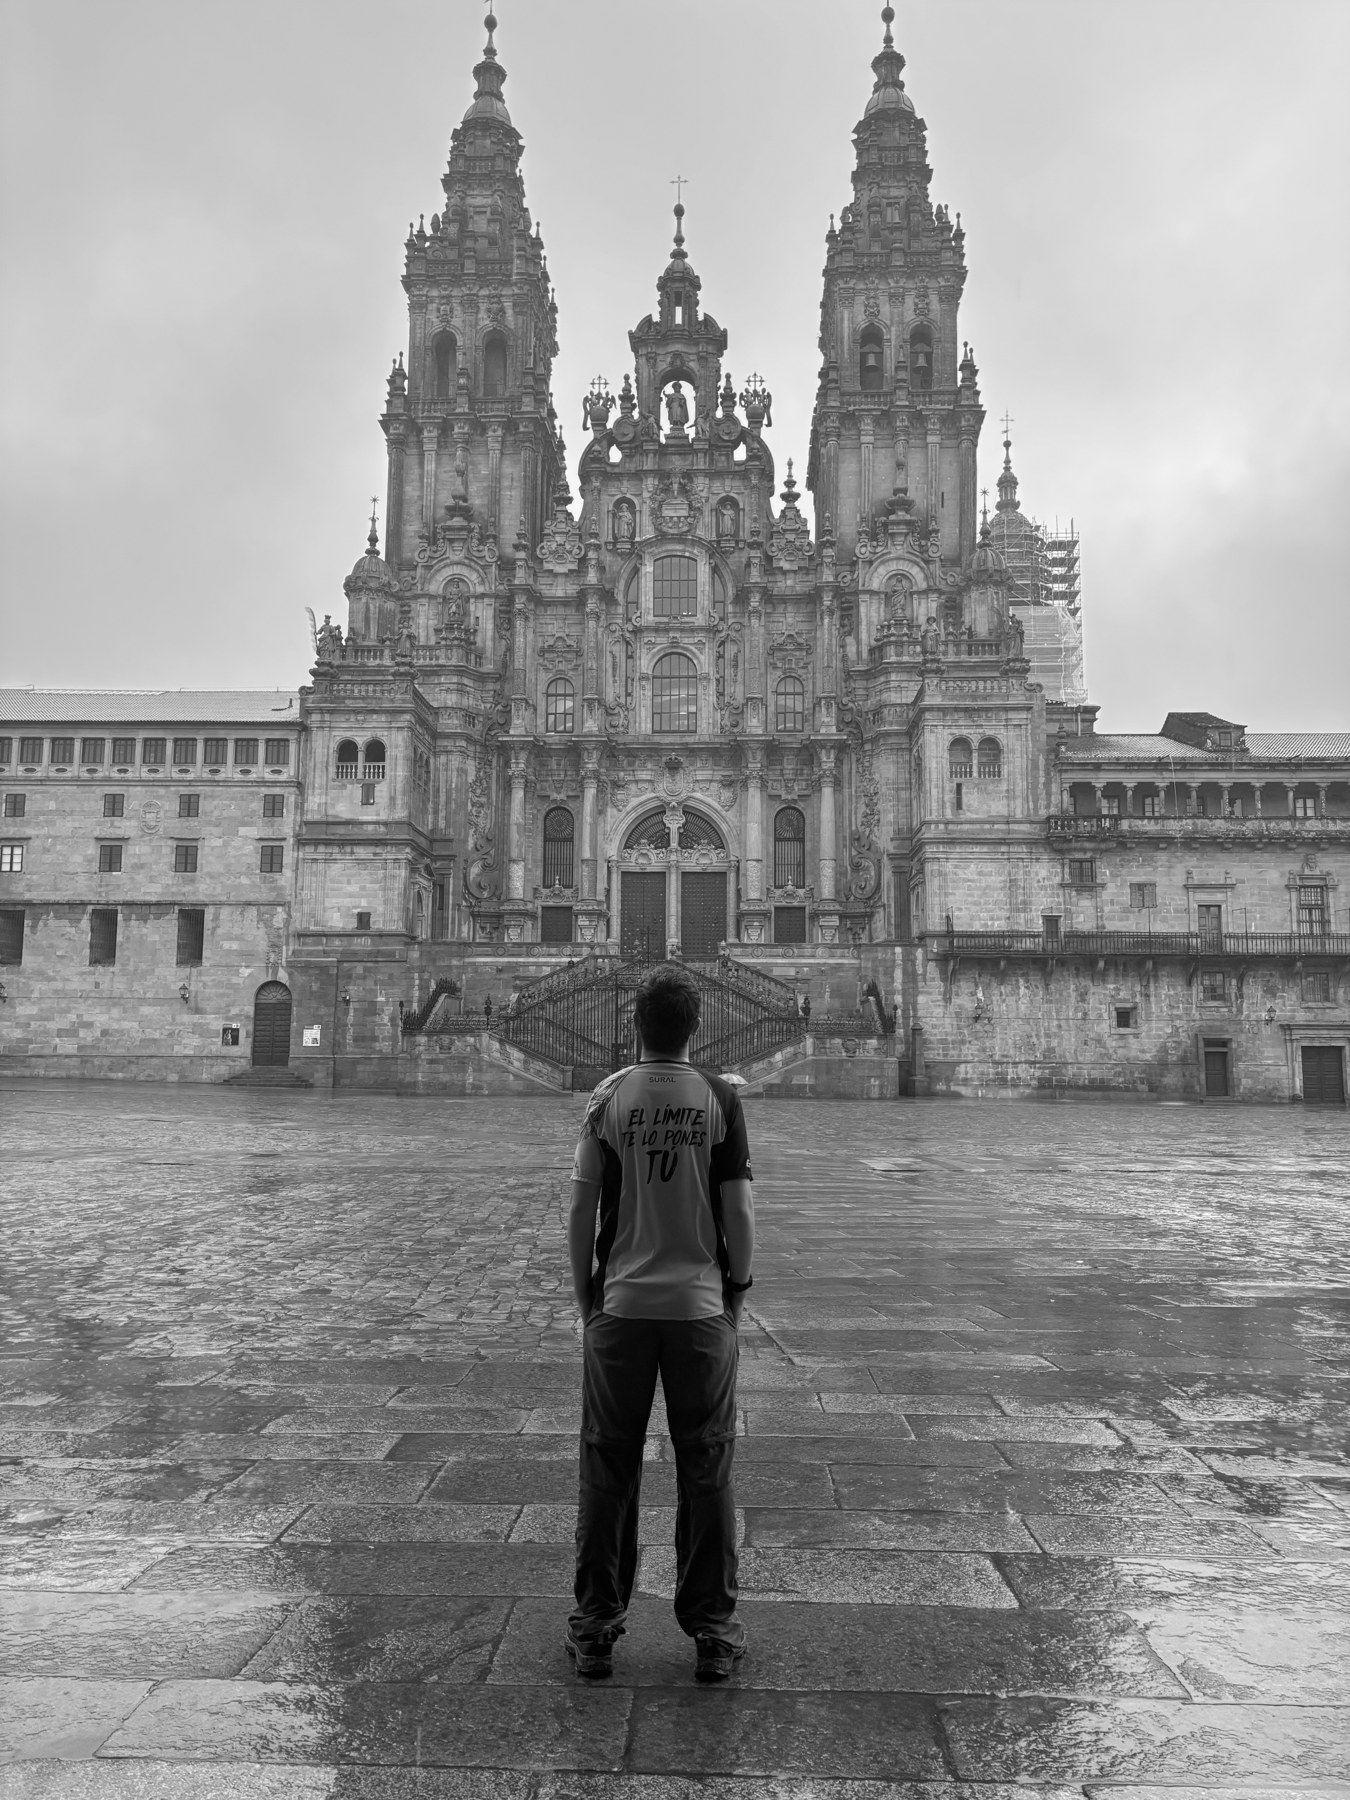
\includegraphics[height=0.82\textheight,keepaspectratio]{figuras/perfil/obradoiro_2026_bn.jpg}
            \end{center}
        \end{column}
        \begin{column}{0.6\textwidth}
            \vspace{-0.2cm}
            \begin{itemize}
                \setlength\itemsep{1em}
                \item \textbf{Ingeniería Informática} \\ 
                Universidad Pablo de Olavide (Sevilla).
                
                \item \textbf{Erasmus en HPC} \\ 
                LUT University (Finlandia).
                
                \item \textbf{Graduate Research Assistant} \\ 
                Grupo de investigación SynergIA.
                
                \item \textbf{Software Engineer} \\ 
                NTT Data.
            \end{itemize}
        \end{column}
    \end{columns}
\end{frame}

\begin{frame}[plain]{Guión general}
    \vspace{0.25cm}
    \Large
    \textbf{¿Cuál es el límite de Python cuando nos enfrentamos a problemas de alta intensidad computacional en bioinformática?}

    \vspace{0.9cm}
    \noindent\begin{tikzpicture}[x=\linewidth]
        \path (0,0) -- (1,0);
        \draw[black!20, line width=1.2pt] (0.1,0) -- (0.9,0);
        \node[circle, fill=blue!75!black, text=white, font=\bfseries, minimum size=0.75cm, inner sep=0pt] at (0.1,0) {1};
        \node[align=center, text=black!82, font=\small] at (0.1,-1) {Problemas\\y algoritmos};
        \node[circle, fill=teal!70!black, text=white, font=\bfseries, minimum size=0.75cm, inner sep=0pt] at (0.3,0) {2};
        \node[align=center, text=black!82, font=\small] at (0.3,-1) {Implementación\\real};
        \node[circle, fill=violet!75!black, text=white, font=\bfseries, minimum size=0.75cm, inner sep=0pt] at (0.5,0) {3};
        \node[align=center, text=black!82, font=\small] at (0.5,-1) {Estrategia\\experimental};
        \node[circle, fill=green!55!black, text=white, font=\bfseries, minimum size=0.75cm, inner sep=0pt] at (0.7,0) {4};
        \node[align=center, text=black!82, font=\small] at (0.7,-1) {Resultados\\estadísticos};
        \node[circle, fill=orange!85!black, text=white, font=\bfseries, minimum size=0.75cm, inner sep=0pt] at (0.9,0) {5};
        \node[align=center, text=black!82, font=\small] at (0.9,-1) {Conclusiones\\e ingeniería};
    \end{tikzpicture}
\end{frame}

% --- SECCIÓN 1: INTRODUCCIÓN Y ALGORITMOS ---
\begin{frame}[plain]
    \begin{tikzpicture}[remember picture,overlay]
        \fill[black!2] (current page.south west) rectangle (current page.north east);
        \fill[blue!72!black] (current page.north west) rectangle ([xshift=0.36cm]current page.south west);
        \fill[blue!72!black] ([xshift=0.36cm]current page.south west) rectangle ([yshift=0.16cm]current page.south east);
        \node[anchor=west, text=blue!72!black, font=\bfseries\Large] at ([xshift=1.25cm,yshift=-1.4cm]current page.north west) {BLOQUE 1/5};
        \node[anchor=west, align=left, text width=13.5cm, text=black, font=\bfseries\fontsize{24}{28}\selectfont] at ([xshift=1.25cm,yshift=-3.35cm]current page.north west) {El reto de la intensidad\\computacional};
        \draw[blue!72!black, line width=1pt] ([xshift=1.25cm,yshift=-5.25cm]current page.north west) -- ([xshift=10.9cm,yshift=-5.25cm]current page.north west);
        \node[anchor=west, align=left, text width=13.5cm, text=black!65, font=\large] at ([xshift=1.25cm,yshift=-6.25cm]current page.north west) {Contexto biológico, formulación matemática y el cuello de botella del GIL.};
    \end{tikzpicture}
\end{frame}

\section{El reto de la intensidad computacional en bioinformática}

\begin{frame}{Contexto biológico: la matriz de expresión génica}
    \begin{columns}
        \begin{column}{0.48\textwidth}
            \begin{center}
            \begin{tikzpicture}[scale=0.5]
                \foreach \r/\vals in {0/{9,8,2,7,1,8},1/{2,3,9,1,8,2},2/{8,9,1,8,2,7},3/{5,4,5,6,4,5},4/{1,2,8,2,9,1},5/{7,8,3,9,2,8}} {
                    \foreach \v [count=\c from 0] in \vals {
                        \pgfmathsetmacro{\pct}{\v*10}
                        \fill[red!\pct!blue!60] (\c,-\r) rectangle ++(1,-1);
                        \draw[white, line width=0.6pt] (\c,-\r) rectangle ++(1,-1);
                    }
                    \pgfmathtruncatemacro{\g}{\r+1}
                    \node[anchor=east, font=\scriptsize] at (0,-\r-0.5) {Gen \g};
                }
                \foreach \r in {0,2,5} {
                    \draw[black, line width=1.6pt] (0,-\r) rectangle ++(6,-1);
                }
                \foreach \c in {1,...,6} {
                    \node[font=\scriptsize] at (\c-0.5,0.55) {M\c};
                }
                \fill[red!100!blue!60] (0.2,-6.7) rectangle ++(0.5,-0.5);
                \node[anchor=west, font=\scriptsize] at (0.75,-6.95) {alta};
                \fill[red!10!blue!60] (3.2,-6.7) rectangle ++(0.5,-0.5);
                \node[anchor=west, font=\scriptsize] at (3.75,-6.95) {baja};
            \end{tikzpicture}
            \end{center}
        \end{column}
        \begin{column}{0.52\textwidth}
            \begin{itemize}
                \setlength\itemsep{0.7em}
                \item \textbf{Fila:} un gen.
                \item \textbf{Columna:} una muestra (paciente, tejido, tratamiento\dots).
                \item \textbf{Celda:} cuánto se \textit{expresa} el gen en esa muestra.
                \item \textbf{Origen:} microarrays y RNA-seq.
                \item \textbf{Escala:} $\sim$20\,000 genes $\times$ cientos o miles de muestras.
            \end{itemize}
        \end{column}
    \end{columns}
\end{frame}


\begin{frame}{Clustering vs.\ Biclustering}
    \begin{columns}[T]
        \begin{column}{0.5\textwidth}
            \centering
            \textbf{Clustering}\\[0.3em]
            \begin{tikzpicture}[scale=0.38]
                \foreach \r in {0,...,5} \foreach \c in {0,...,7} {
                    \draw[gray!50, fill=gray!8] (\c,-\r) rectangle ++(1,-1);
                }
                \foreach \r in {0,2,5} \foreach \c in {0,...,7} {
                    \draw[gray!50, fill=blue!45] (\c,-\r) rectangle ++(1,-1);
                }
            \end{tikzpicture}\\[0.3em]
            {\small Genes parecidos en \textbf{todas} las muestras}
        \end{column}
        \begin{column}{0.5\textwidth}
            \centering
            \textbf{Biclustering}\\[0.3em]
            \begin{tikzpicture}[scale=0.38]
                \foreach \r in {0,...,5} \foreach \c in {0,...,7} {
                    \draw[gray!50, fill=gray!8] (\c,-\r) rectangle ++(1,-1);
                }
                \foreach \r in {0,2,5} \foreach \c in {1,3,4,6} {
                    \draw[gray!50, fill=orange!70] (\c,-\r) rectangle ++(1,-1);
                }
            \end{tikzpicture}\\[0.3em]
            {\small Genes parecidos \textbf{solo en algunas} muestras}
        \end{column}
    \end{columns}
    \vspace{0.5cm}
    \begin{itemize}
        \item \textbf{Para qué sirve:} módulos de genes co-regulados, subtipos de enfermedad, biomarcadores, respuesta a fármacos.
    \end{itemize}
\end{frame}


\begin{frame}{BiBit y BCCA: ¿qué buscan?}
    \begin{columns}[T]
        \begin{column}{0.5\textwidth}
            \textbf{BiBit} {\footnotesize(Rodríguez-Baena et al., 2011)}
            \begin{itemize}
                \item Datos \textbf{binarios}: gen activo / inactivo.
                \item Busca genes que se \textbf{encienden a la vez} en las mismas muestras.
            \end{itemize}
        \end{column}
        \begin{column}{0.5\textwidth}
            \textbf{BCCA} {\footnotesize(Bhattacharya y De, 2009)}
            \begin{itemize}
                \item Datos \textbf{continuos}: nivel de expresión.
                \item Busca genes que \textbf{suben y bajan juntos} (correlación alta).
            \end{itemize}
        \end{column}
    \end{columns}
\end{frame}

\begin{frame}{Desafíos del biclustering}
    \begin{columns}[T]
        \begin{column}{0.5\textwidth}
            \begin{center}
            \textbf{Del problema}\\[0.6em]
            \begin{tikzpicture}[
                box/.style={draw=gray!70, fill=gray!15, rounded corners=1ex, very thick, minimum width=4.6cm, minimum height=0.8cm, align=center, font=\normalsize\bfseries}
            ]
                \node[box] at (0, 0) {Complejidad de los datos};
                \node[box] at (0, -1.2) {Métodos};
                \node[box] at (0, -2.4) {Validación};
            \end{tikzpicture}
            \end{center}
        \end{column}
        \begin{column}{0.5\textwidth}
            \begin{center}
            \textbf{De los datos}\\[0.6em]
            \begin{tikzpicture}[
                box/.style={draw=gray!70, fill=gray!15, rounded corners=1ex, very thick, minimum width=4.6cm, minimum height=0.8cm, align=center, font=\normalsize\bfseries}
            ]
                \node[box] at (0, 0) {Volumen};
                \node[box] at (0, -1.2) {Variedad};
                \node[box] at (0, -2.4) {Veracidad};
            \end{tikzpicture}
            \end{center}
        \end{column}
    \end{columns}
\end{frame}


\begin{frame}{Limitaciones del Big Data (Hadoop/Spark)}
    \begin{center}
    \begin{tikzpicture}[
        box/.style={draw=gray!70, fill=gray!15, rounded corners=1ex, very thick, minimum width=7cm, minimum height=0.8cm, align=center, font=\normalsize\bfseries}
    ]
        \node[box] (b1) at (0, 0) {Arranque en frío};
        \node[box] (b2) at (0, -1.2) {Incompatibilidad con MapReduce};
        \node[box] (b3) at (0, -2.4) {Sincronización de red};
        \node[box] (b4) at (0, -3.6) {Cuello de botella en disco};
    \end{tikzpicture}
    \end{center}
\end{frame}

\begin{frame}{Los algoritmos: BiBit y BCCA}
    \begin{columns}
        \begin{column}{0.5\textwidth}
            \textbf{BiBit (Binarios):}
            \begin{itemize}
                \item Lógica \textit{bitwise}
                \item Patrones frecuentes
                \item Alta eficiencia
            \end{itemize}
        \end{column}
        \begin{column}{0.5\textwidth}
            \textbf{BCCA (Continuos):}
            \begin{itemize}
                \item Correlación numérica
                \item Alta carga aritmética
                \item Refinamiento destructivo
            \end{itemize}
        \end{column}
    \end{columns}
    \vspace{0.4cm}
    \begin{alertblock}{Cuello de Botella}
        Sobrecarga del intérprete y contención del GIL.
    \end{alertblock}
\end{frame}

\begin{frame}{Complejidad algorítmica}
    \begin{table}
        \centering
        \renewcommand{\arraystretch}{1.5}
        \resizebox{0.85\textwidth}{!}{
        \begin{tabular}{@{}lccc@{}}
            \toprule
            \textbf{Escenario} & \textbf{BiBit} & \textbf{BCCA} & \textbf{Algoritmos Biclustering} \\ \midrule
            \textbf{Mejor Caso}    & $\mathcal{O}(N \cdot M)$ & $\mathcal{O}(N^3)$ & $\mathcal{O}(N \cdot M)$ \\
            \textbf{Caso Promedio} & $\mathcal{O}(N^2)$ & $\mathcal{O}(N^4)$ & Heurísticas polinómicas \\
            \textbf{Peor Caso}     & $\mathcal{O}(N^2 \cdot M)$ & $\mathcal{O}(N^4)$ & \textbf{NP-Hard ($\mathcal{O}(2^N)$)} \\
            \bottomrule
        \end{tabular}
        }
    \end{table}
\end{frame}

\begin{frame}{Proyección del coste: BiBit}
    \begin{center}
        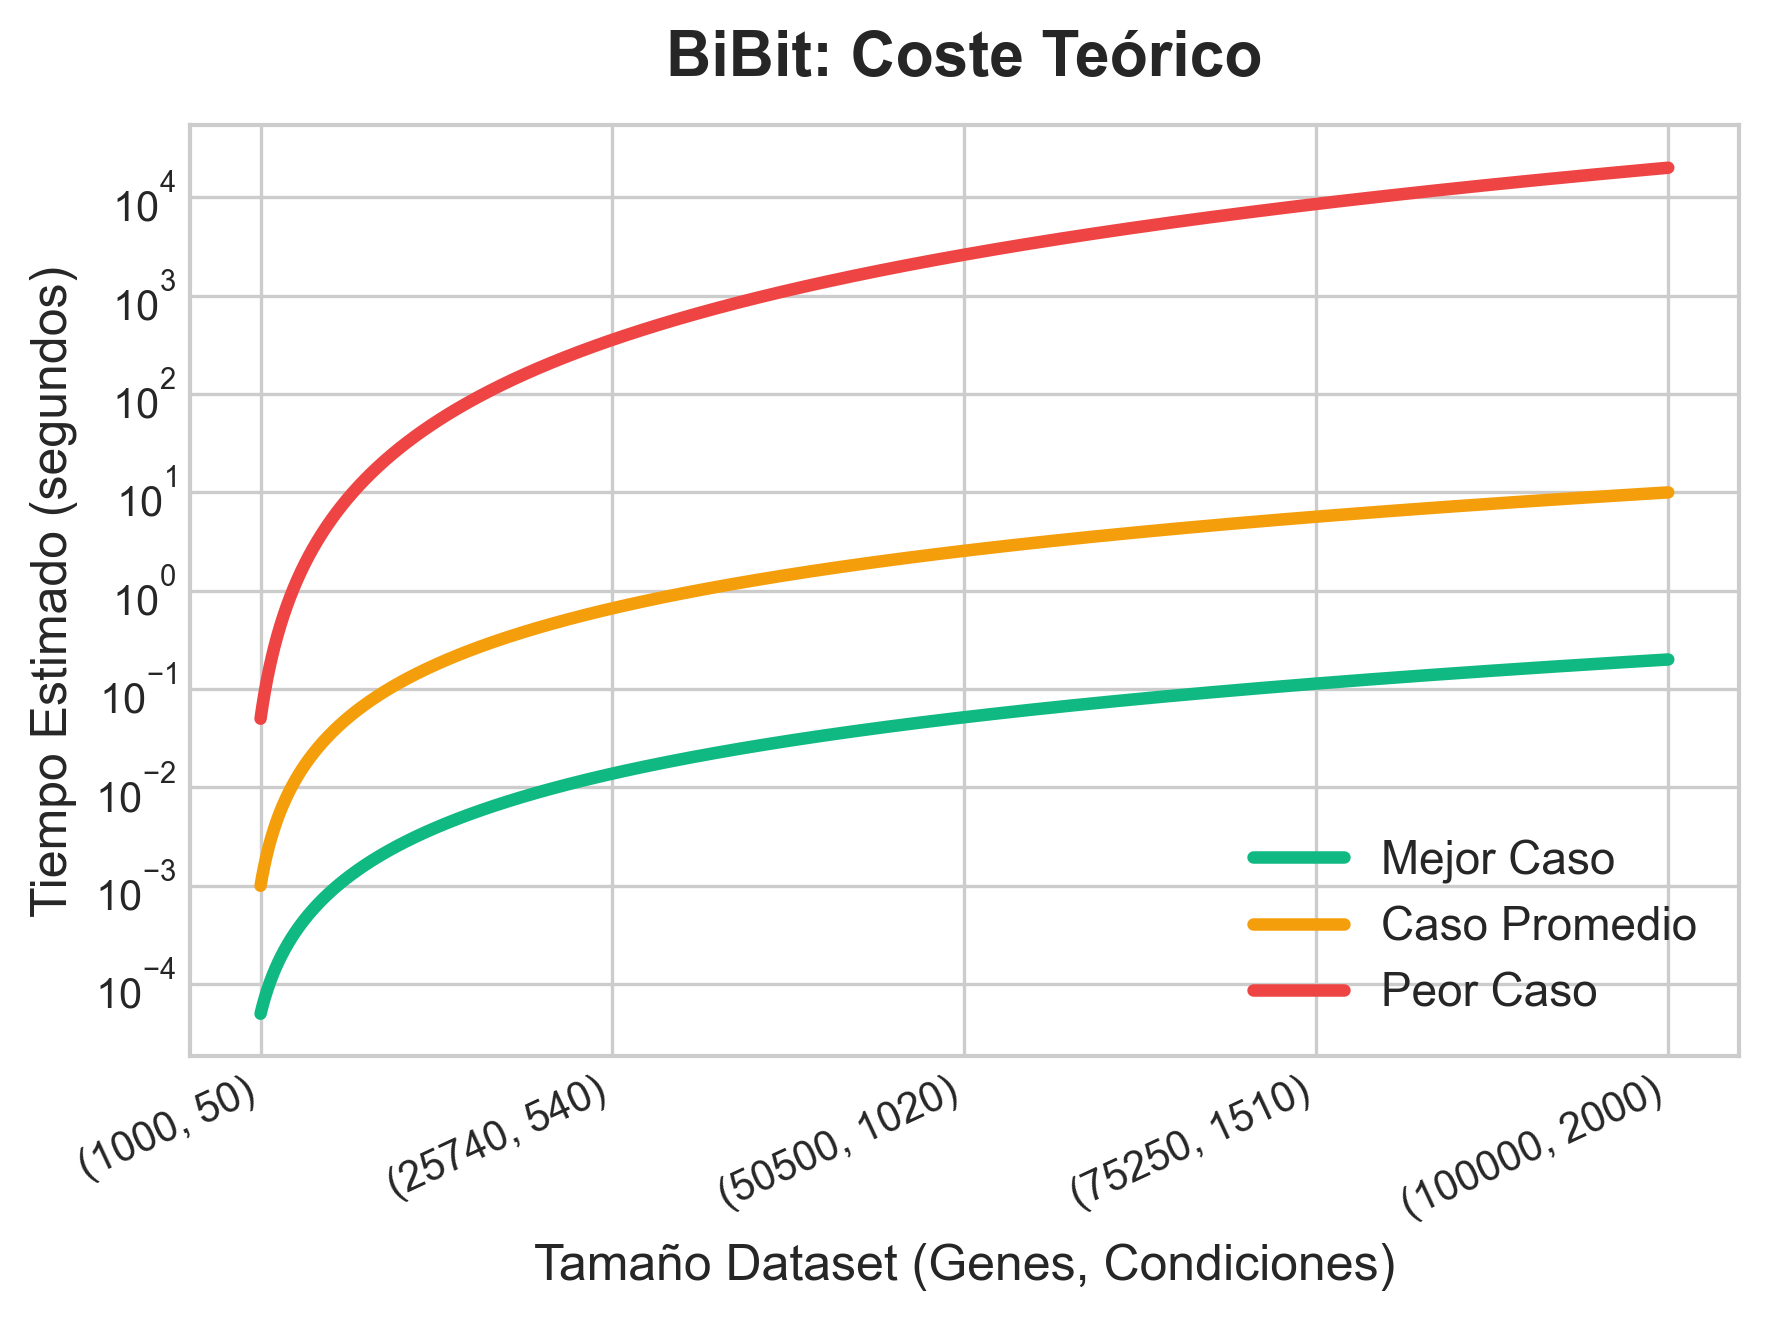
\includegraphics[height=0.75\textheight,keepaspectratio]{figuras/complejidad/bibit_complejidad.png}
    \end{center}
    \vspace{-0.3cm}
    \begin{itemize}
        \item \textbf{BiBit ($\mathcal{O}(N^2)$):} Crecimiento polinómico asimilable.
    \end{itemize}
\end{frame}

\begin{frame}{Proyección del coste: BCCA}
    \begin{center}
        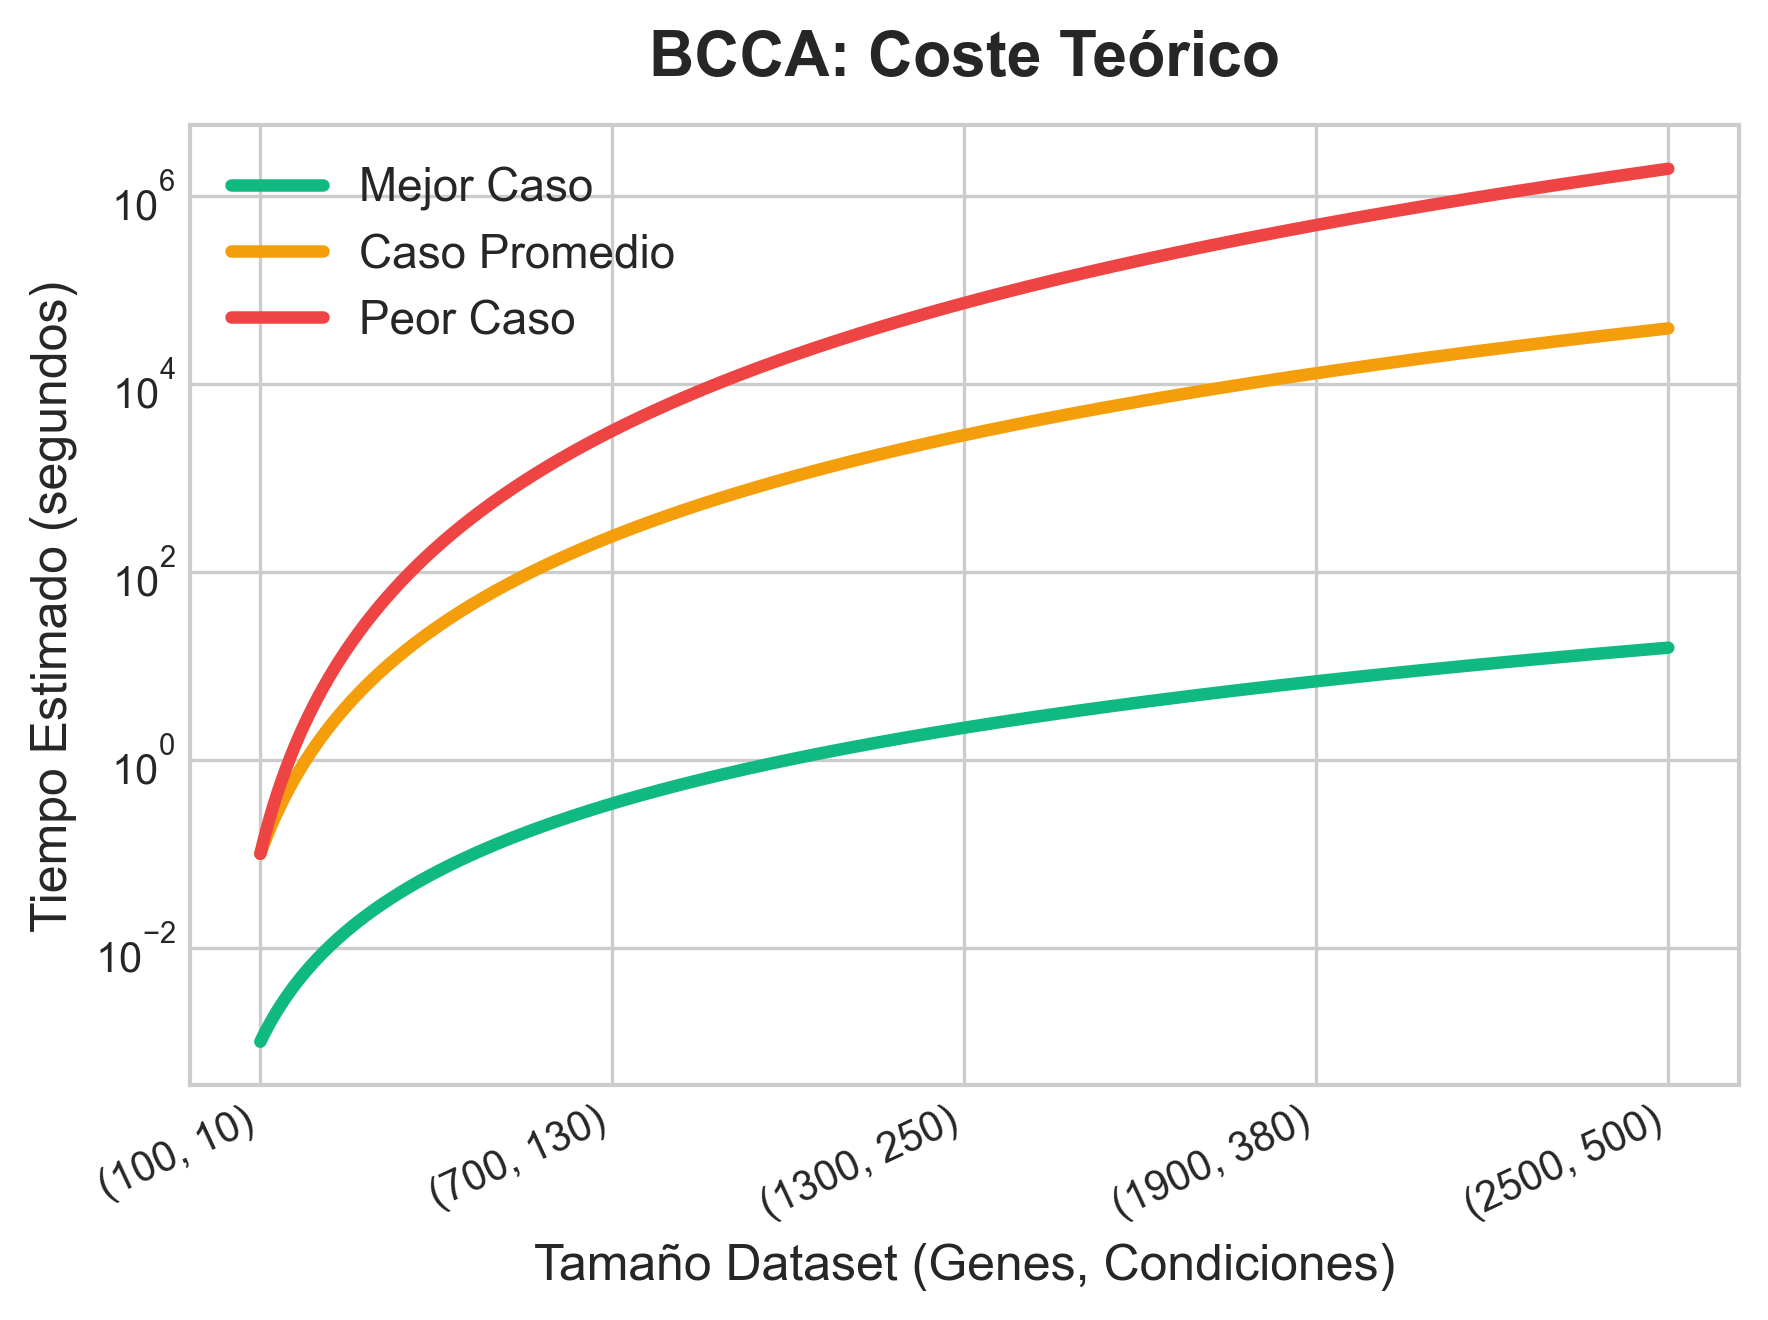
\includegraphics[height=0.75\textheight,keepaspectratio]{figuras/complejidad/bcca_complejidad.png}
    \end{center}
    \vspace{-0.3cm}
    \begin{itemize}
        \item \textbf{BCCA ($\mathcal{O}(N^4)$):} Saturación rápida en CPUs.
    \end{itemize}
\end{frame}

\begin{frame}{Proyección del coste: NP-Hard}
    \begin{center}
        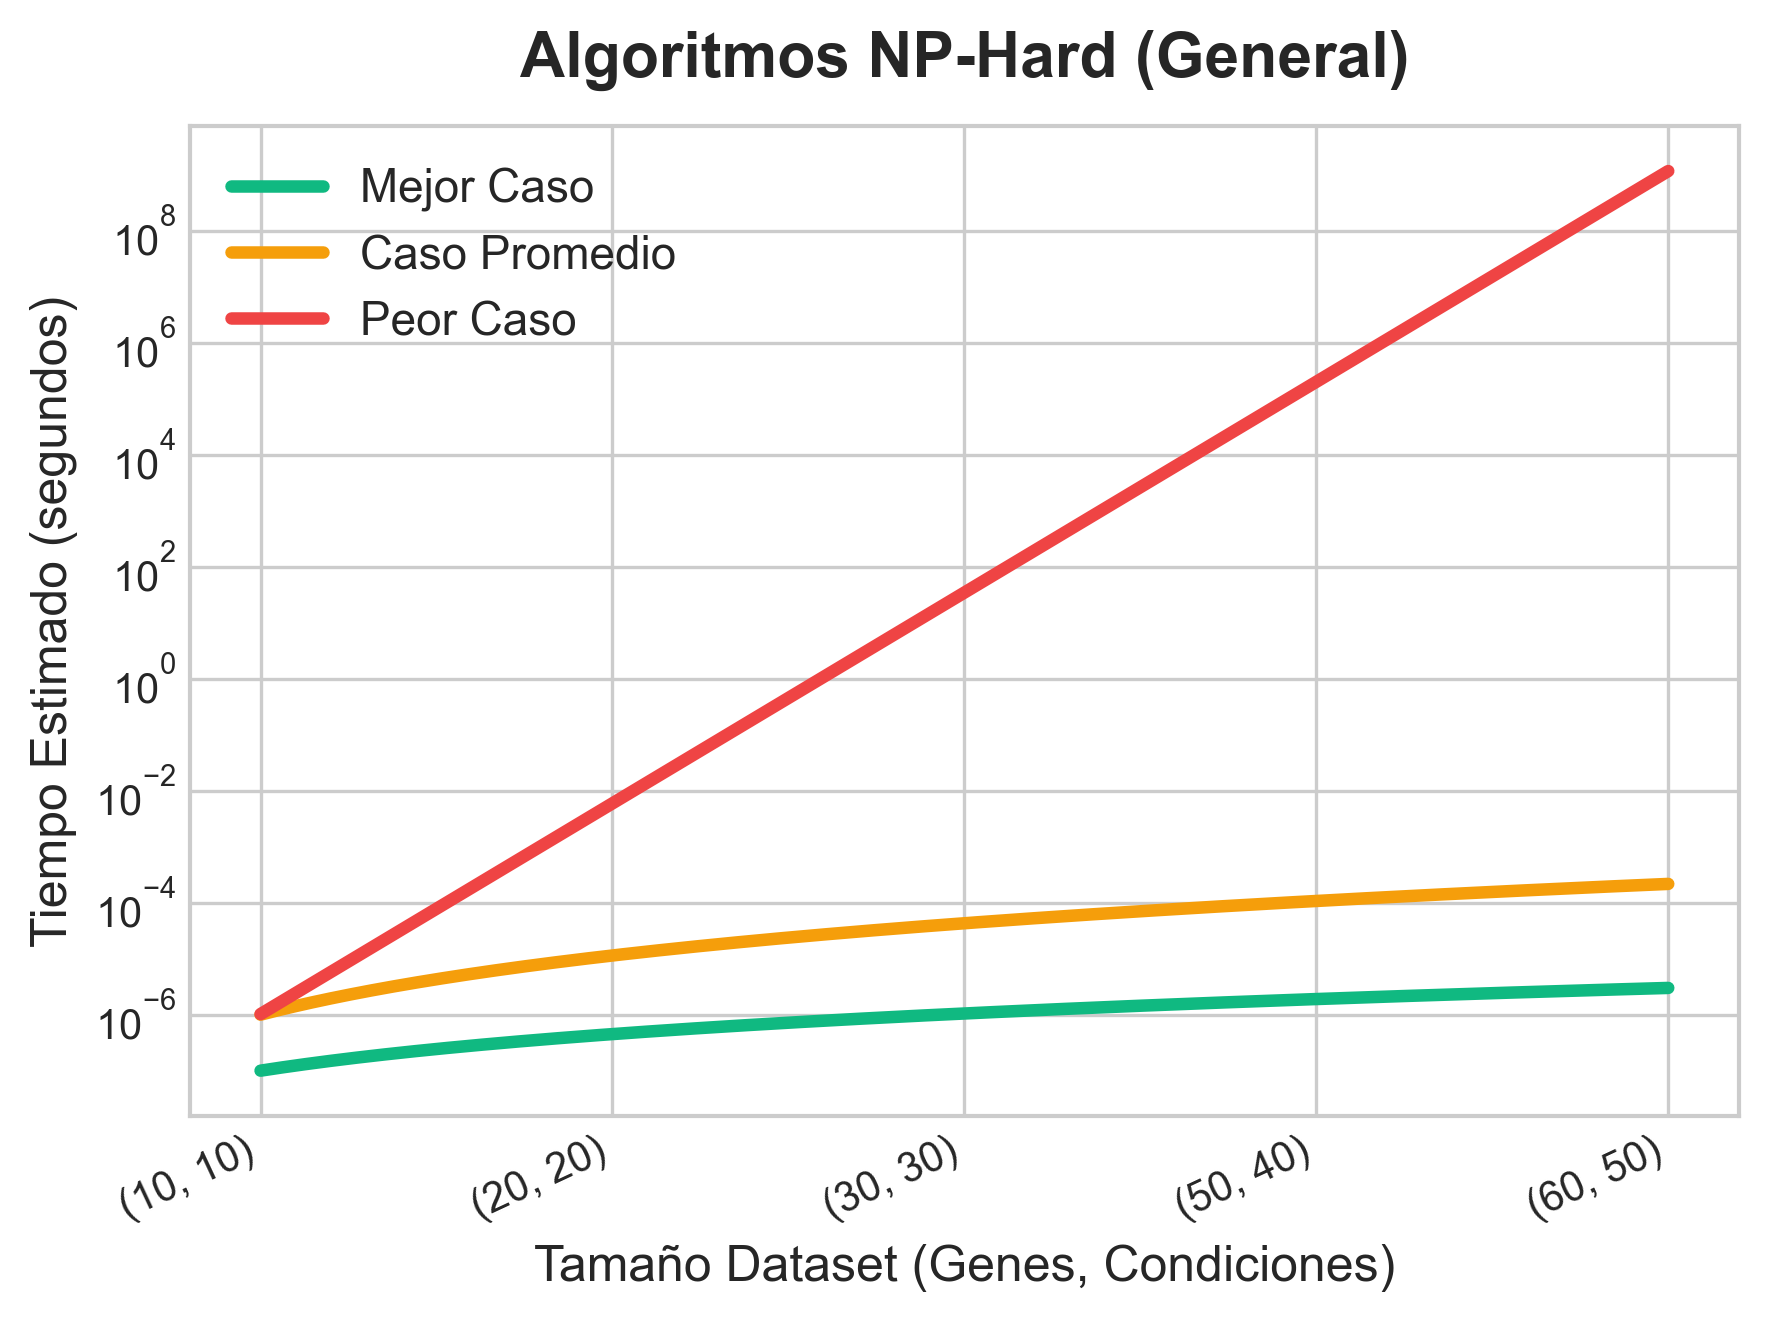
\includegraphics[height=0.75\textheight,keepaspectratio]{figuras/complejidad/nphard_complejidad.png}
    \end{center}
    \vspace{-0.3cm}
    \begin{itemize}
        \item \textbf{NP-Hard ($\mathcal{O}(2^N)$):} Explosión computacional inmediata.
    \end{itemize}
\end{frame}

\begin{frame}[fragile]{Algoritmo BiBit: extracción y formación}
    \textbf{Fase 1: Patrones Frecuentes}
    \begin{itemize}
        \item Operaciones \textit{bitwise AND} entre filas.
        \item Conteo rápido (\textit{popcount}).
    \end{itemize}
    \vspace{0.3cm}
    \textbf{Fase 2: Inclusión de Biclústers}
    \begin{itemize}
        \item Validación estricta.
        \item Consolidación de filas.
    \end{itemize}
\end{frame}

\begin{frame}{Algoritmo BiBit: fase 1, extracción de patrones frecuentes}
    \begin{center}
        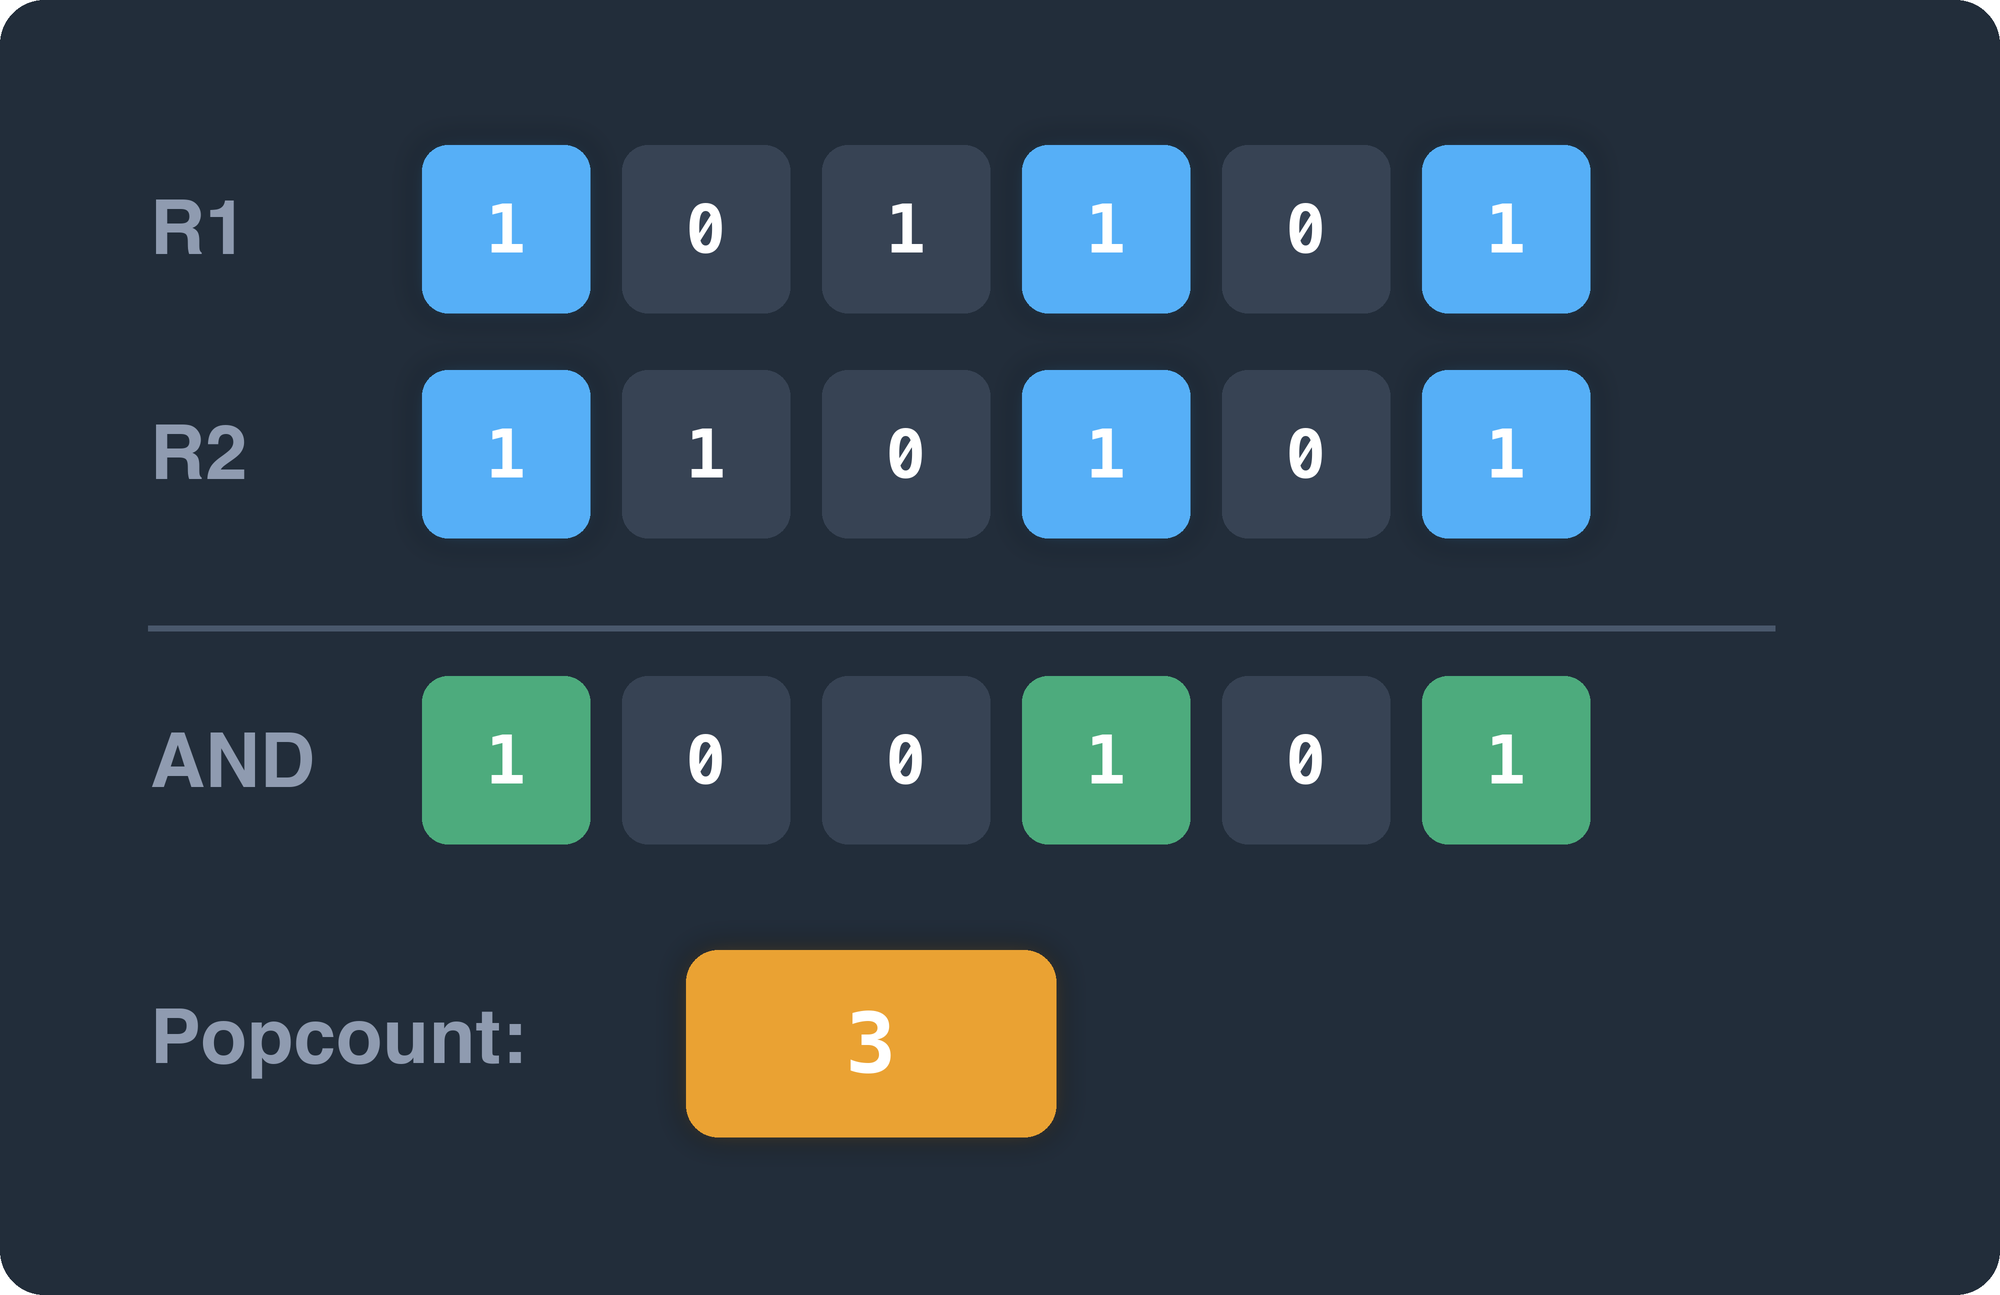
\includegraphics[width=\textwidth,height=0.86\textheight,keepaspectratio]{figuras/bibit/Imagen_1_v3.png}
    \end{center}
\end{frame}

\begin{frame}{Algoritmo BiBit: fase 2, formación e inclusión de biclústeres}
    \begin{center}
        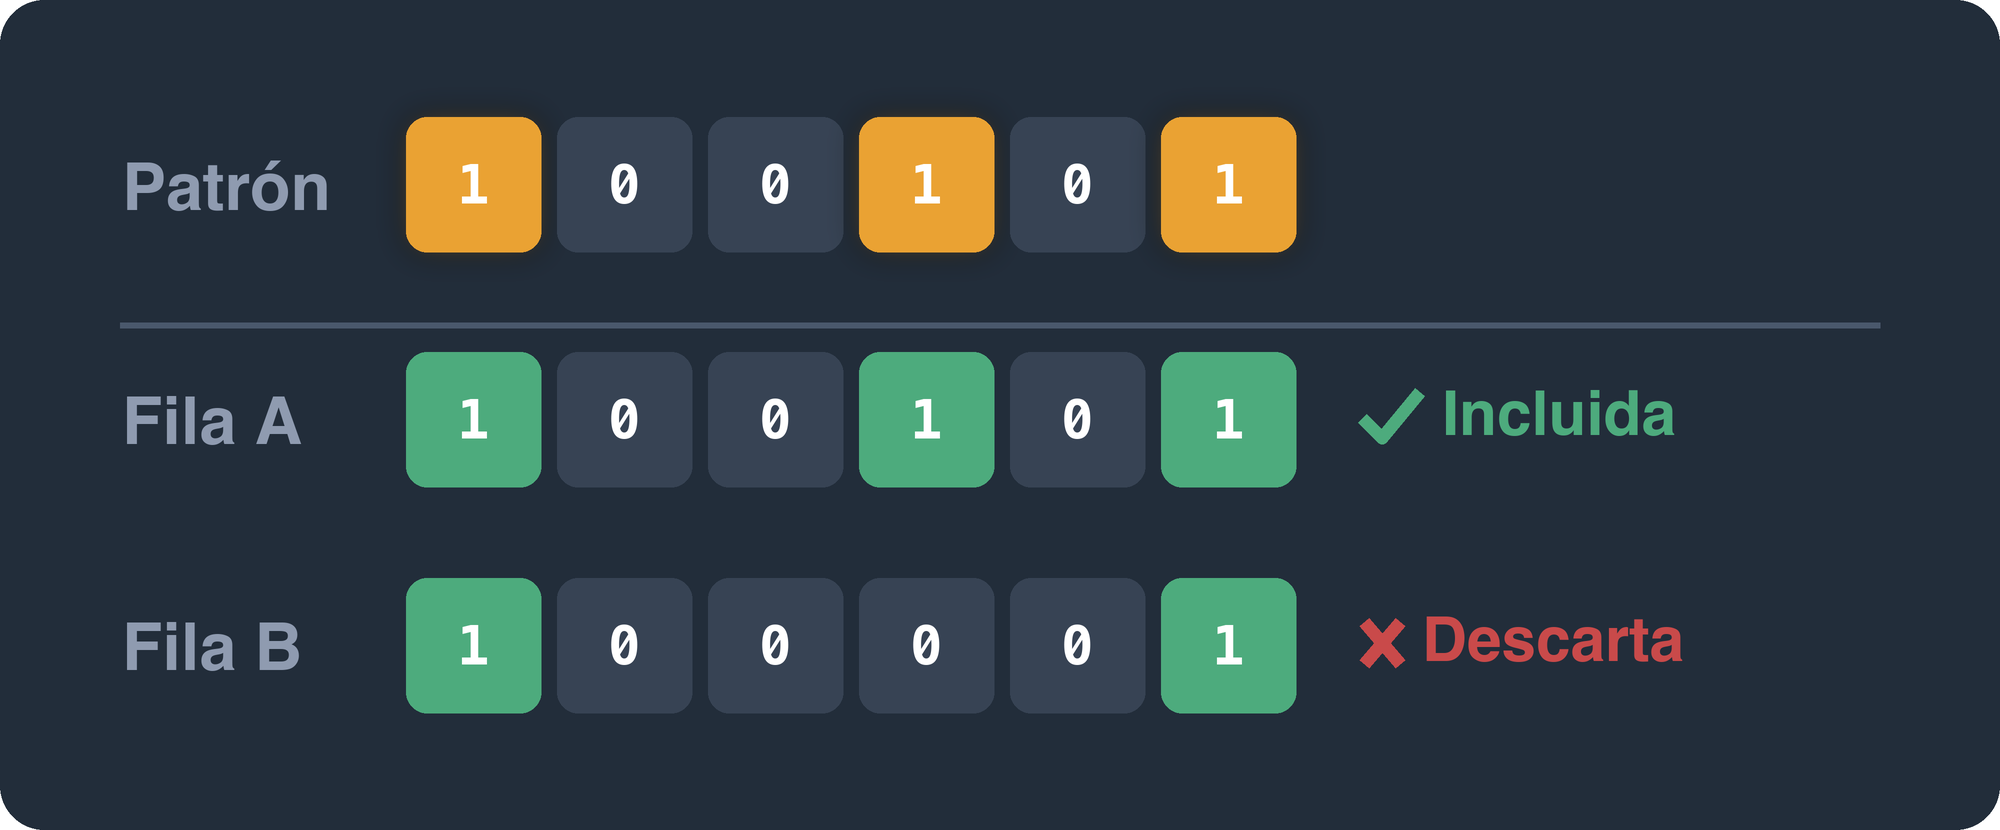
\includegraphics[width=\textwidth,height=0.86\textheight,keepaspectratio]{figuras/bibit/Imagen_2_v3.png}
    \end{center}
\end{frame}

\begin{frame}{Algoritmo BCCA: filtrado por correlación}
    \begin{itemize}
        \item \textbf{Enfoque destructivo:} Matriz inicial completa.
        \item \textbf{Poda progresiva:} eliminación de columnas.
        \item \textbf{Convergencia:} biclúster candidato consolidado.
    \end{itemize}
\end{frame}

\begin{frame}{Algoritmo BCCA}
    \begin{center}
        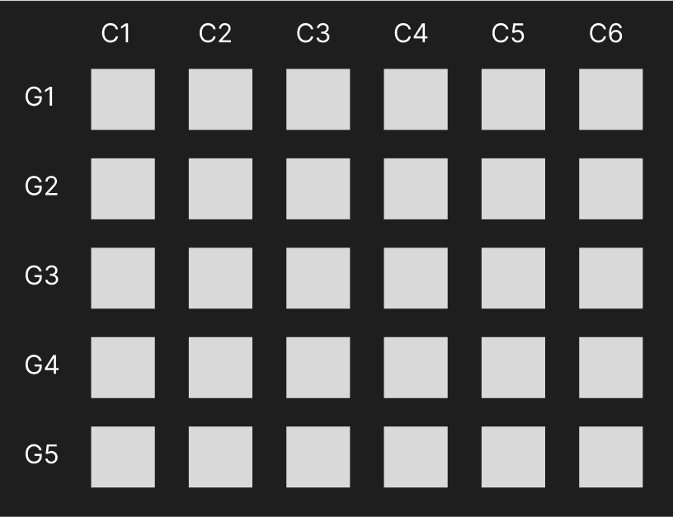
\includegraphics[width=0.85\textwidth,height=0.8\textheight,keepaspectratio]{figuras/bcca/Imagen_1.png}
    \end{center}
\end{frame}
\begin{frame}{Algoritmo BCCA}
    \begin{center}
        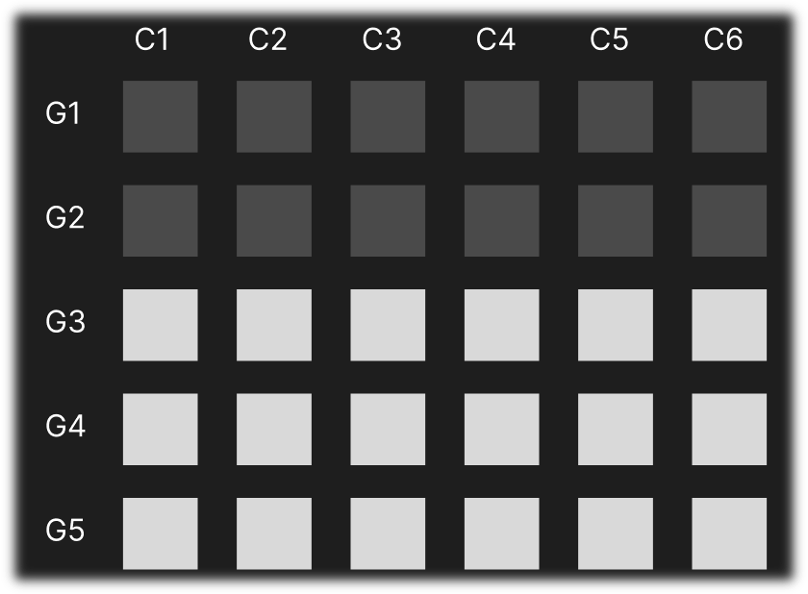
\includegraphics[width=0.85\textwidth,height=0.8\textheight,keepaspectratio]{figuras/bcca/Imagen_2.png}
    \end{center}
\end{frame}
\begin{frame}{Algoritmo BCCA}
    \begin{center}
        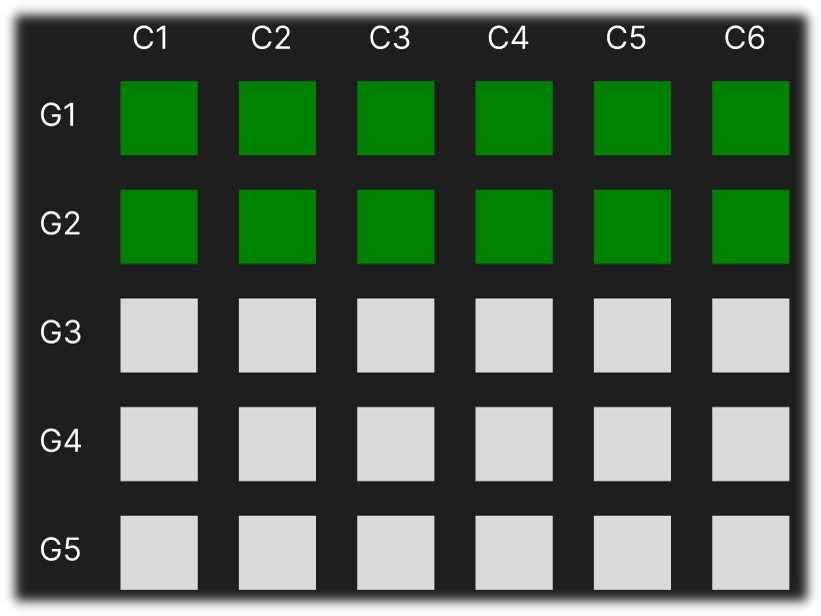
\includegraphics[width=0.85\textwidth,height=0.8\textheight,keepaspectratio]{figuras/bcca/Imagen_3.png}
    \end{center}
\end{frame}
\begin{frame}{Algoritmo BCCA}
    \begin{center}
        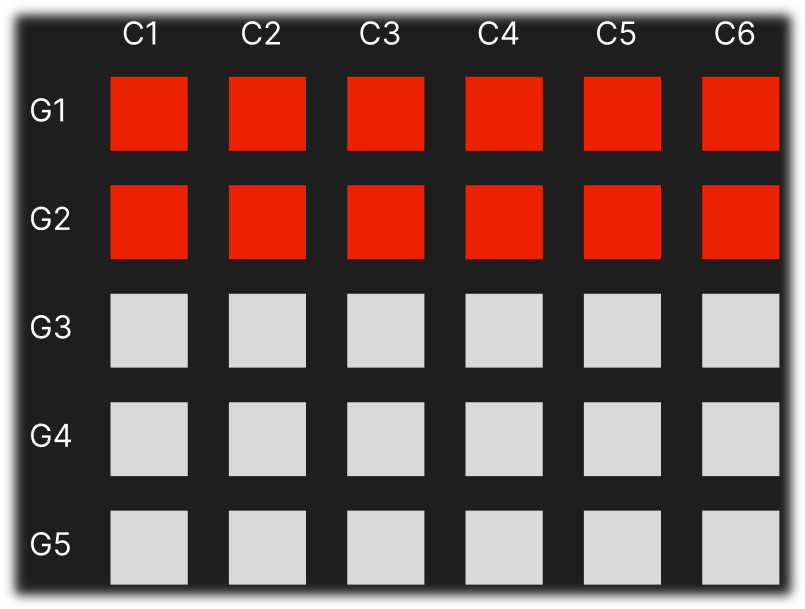
\includegraphics[width=0.85\textwidth,height=0.8\textheight,keepaspectratio]{figuras/bcca/Imagen_4.png}
    \end{center}
\end{frame}
\begin{frame}{Algoritmo BCCA}
    \begin{center}
        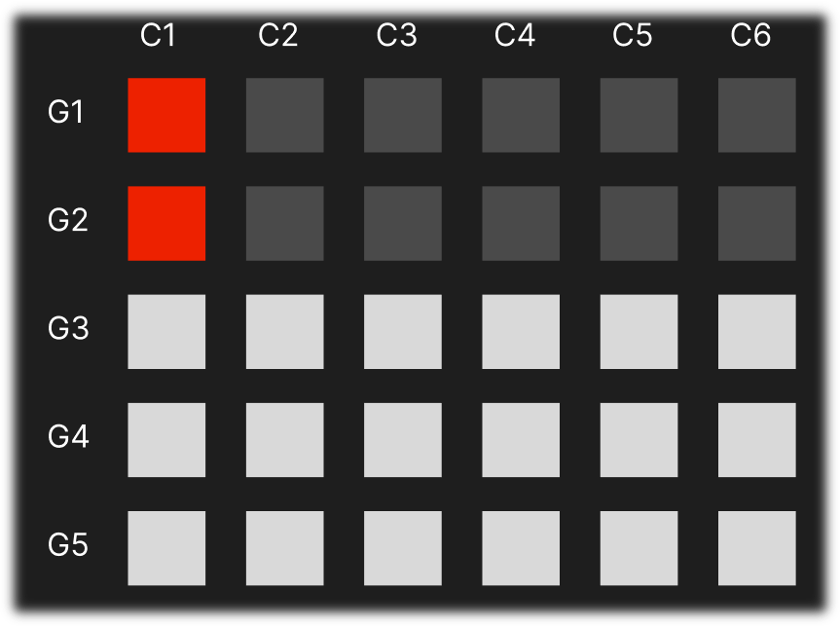
\includegraphics[width=0.85\textwidth,height=0.8\textheight,keepaspectratio]{figuras/bcca/Imagen_5.png}
    \end{center}
\end{frame}
\begin{frame}{Algoritmo BCCA}
    \begin{center}
        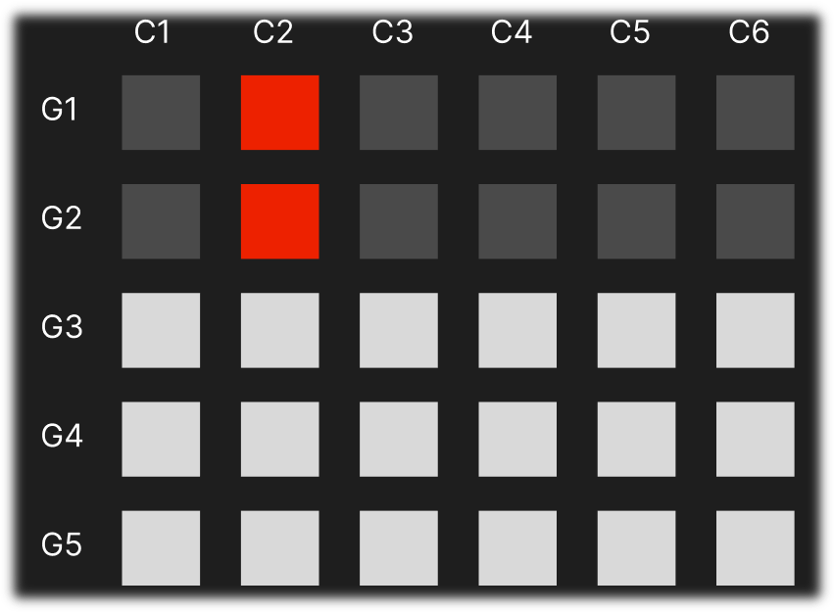
\includegraphics[width=0.85\textwidth,height=0.8\textheight,keepaspectratio]{figuras/bcca/Imagen_6.png}
    \end{center}
\end{frame}
\begin{frame}{Algoritmo BCCA}
    \begin{center}
        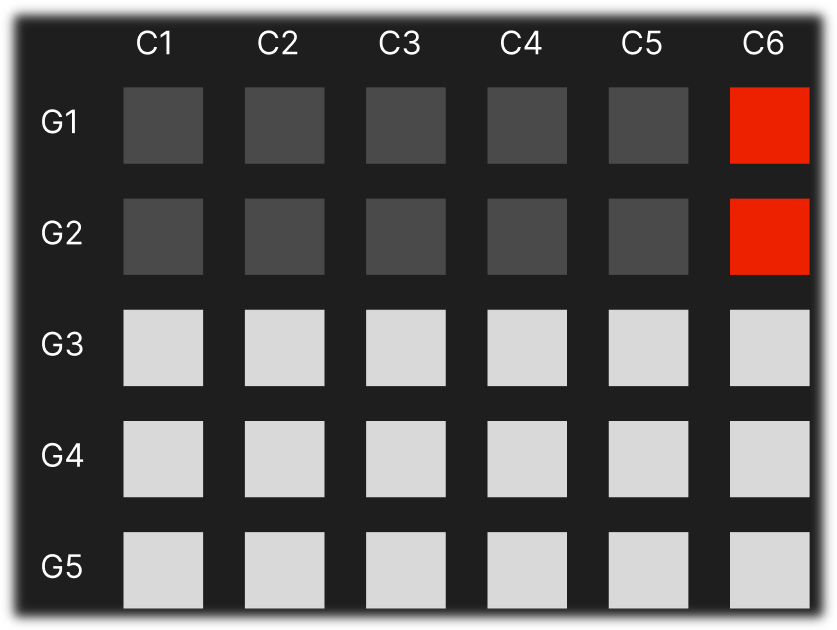
\includegraphics[width=0.85\textwidth,height=0.8\textheight,keepaspectratio]{figuras/bcca/Imagen_7.png}
    \end{center}
\end{frame}
\begin{frame}{Algoritmo BCCA}
    \begin{center}
        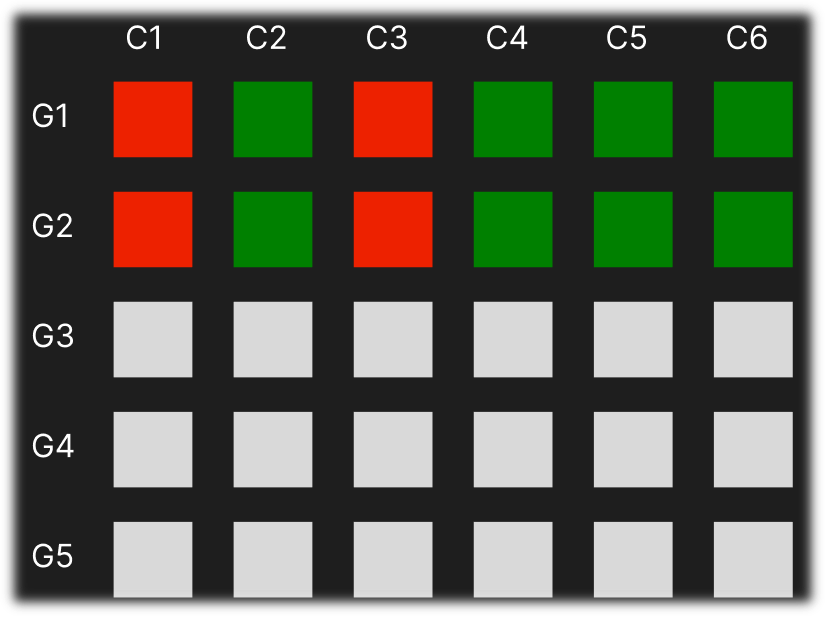
\includegraphics[width=0.85\textwidth,height=0.8\textheight,keepaspectratio]{figuras/bcca/Imagen_8.png}
    \end{center}
\end{frame}
\begin{frame}{Algoritmo BCCA}
    \begin{center}
        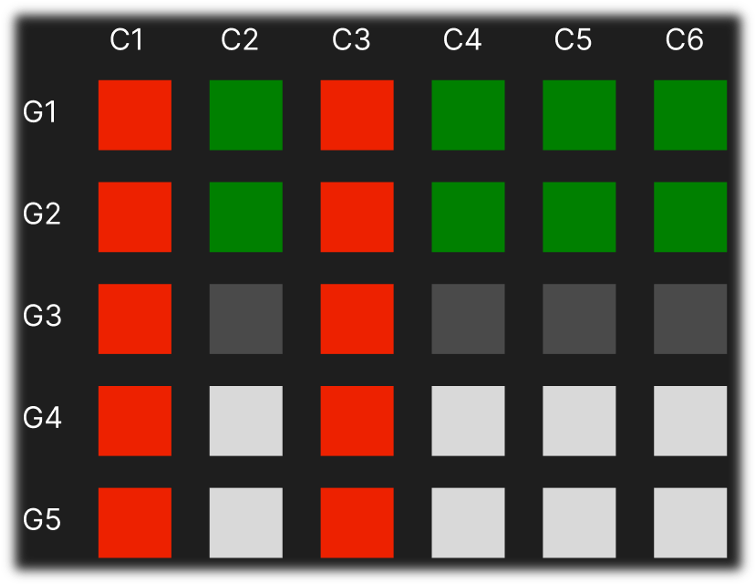
\includegraphics[width=0.85\textwidth,height=0.8\textheight,keepaspectratio]{figuras/bcca/Imagen_9.png}
    \end{center}
\end{frame}
\begin{frame}{Algoritmo BCCA}
    \begin{center}
        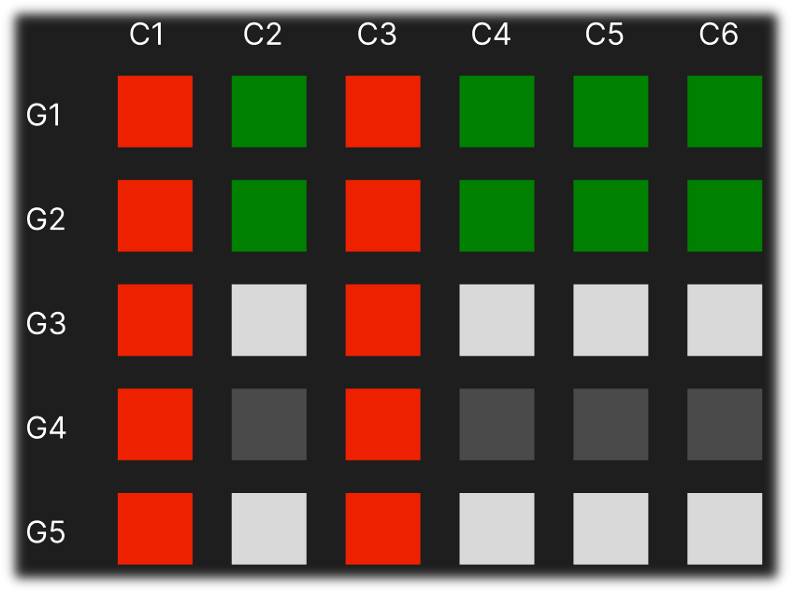
\includegraphics[width=0.85\textwidth,height=0.8\textheight,keepaspectratio]{figuras/bcca/Imagen_10.png}
    \end{center}
\end{frame}
\begin{frame}{Algoritmo BCCA}
    \begin{center}
        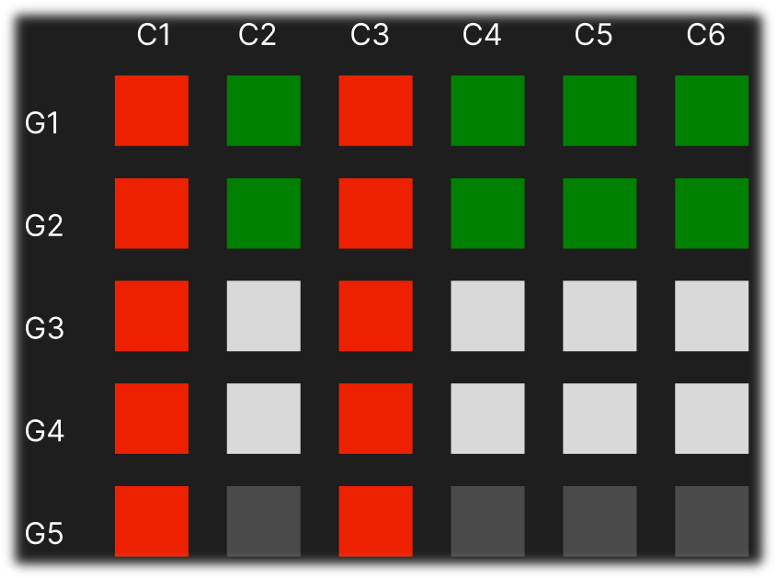
\includegraphics[width=0.85\textwidth,height=0.8\textheight,keepaspectratio]{figuras/bcca/Imagen_11.png}
    \end{center}
\end{frame}
\begin{frame}{Algoritmo BCCA}
    \begin{center}
        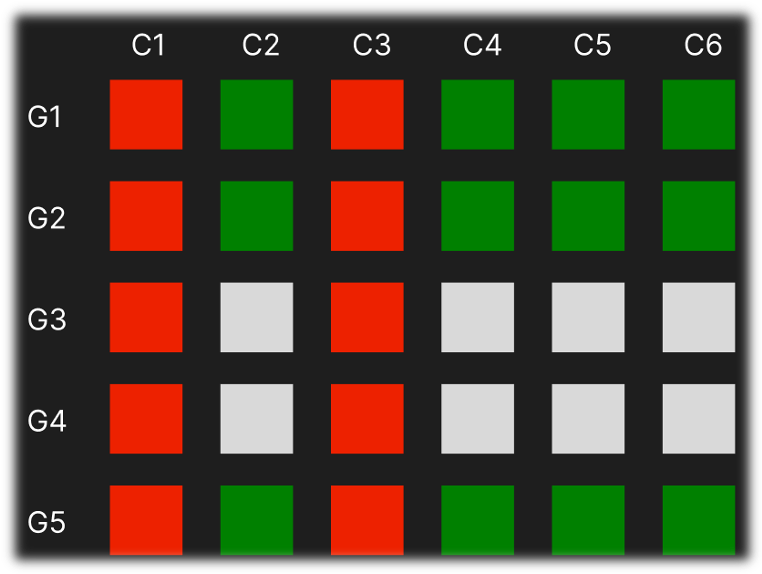
\includegraphics[width=0.85\textwidth,height=0.8\textheight,keepaspectratio]{figuras/bcca/Imagen_12.png}
    \end{center}
\end{frame}
\begin{frame}{Algoritmo BCCA}
    \begin{center}
        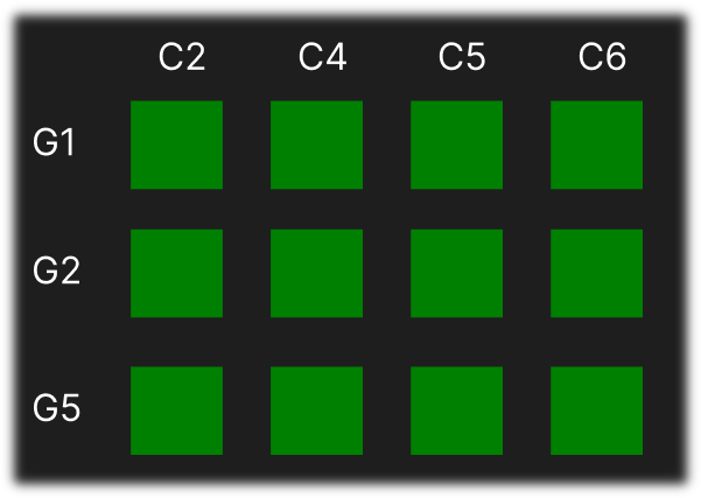
\includegraphics[width=0.85\textwidth,height=0.8\textheight,keepaspectratio]{figuras/bcca/Imagen_13.png}
    \end{center}
\end{frame}

\begin{frame}{Metodología del benchmark}
    \begin{itemize}
        \item \textbf{Aceleración estricta:} speedup frente al secuencial.
        \item \textbf{Trade-off:} complejidad y mantenimiento.
    \end{itemize}
\end{frame}

\begin{frame}{Motor multiparadigma: 6 variantes implementadas}
    \begin{columns}
        \begin{column}{0.5\textwidth}
            \textbf{CPU:}
            \begin{itemize}
                \item Python Secuencial
                \item Python Numba Paralelo
                \item Cython Secuencial
                \item Cython OpenMP
            \end{itemize}
        \end{column}
        \begin{column}{0.5\textwidth}
            \textbf{GPU:}
            \begin{itemize}
                \item Python Numba CUDA
                \item Cython CUDA nativo
            \end{itemize}
        \end{column}
    \end{columns}
\end{frame}

% --- SECCIÓN 2: IMPLEMENTACIÓN REAL ---
\begin{frame}[plain]
    \begin{tikzpicture}[remember picture,overlay]
        \fill[black!2] (current page.south west) rectangle (current page.north east);
        \fill[blue!72!black] (current page.north west) rectangle ([xshift=0.36cm]current page.south west);
        \fill[blue!72!black] ([xshift=0.36cm]current page.south west) rectangle ([yshift=0.16cm]current page.south east);
        \node[anchor=west, text=blue!72!black, font=\bfseries\Large] at ([xshift=1.25cm,yshift=-1.4cm]current page.north west) {BLOQUE 2/5};
        \node[anchor=west, align=left, text width=13.5cm, text=black, font=\bfseries\fontsize{24}{28}\selectfont] at ([xshift=1.25cm,yshift=-3.35cm]current page.north west) {Implementación real};
        \draw[blue!72!black, line width=1pt] ([xshift=1.25cm,yshift=-5.25cm]current page.north west) -- ([xshift=10.9cm,yshift=-5.25cm]current page.north west);
        \node[anchor=west, align=left, text width=13.5cm, text=black!65, font=\large] at ([xshift=1.25cm,yshift=-6.25cm]current page.north west) {Arquitectura multiparadigma, Numba, Cython y optimización en GPU.};
    \end{tikzpicture}
\end{frame}

\section{Implementación real}

\begin{frame}{Implementación teórica: BiBit paralelo}
    \begin{center}
    \begin{tikzpicture}[
        cpubox/.style={draw=blue!60, fill=blue!10, rounded corners=1ex, very thick, minimum width=4.5cm, minimum height=2.8cm, align=center},
        gpubox/.style={draw=orange!60, fill=orange!15, rounded corners=1ex, very thick, minimum width=4.5cm, minimum height=2.8cm, align=center}
    ]
        \node[cpubox] (cpu) at (-3,0) {
            \textbf{CPU} \\[1em]
            Contar y luego rellenar \\[0.4em]
            Reparto equilibrado \\[0.4em]
            Sin \textit{locks}
        };
        
        \node[gpubox] (gpu) at (3,0) {
            \textbf{GPU} \\[1em]
            Mapeo hilo $\rightarrow$ pareja \\[0.4em]
            Ecuación cuadrática \\[0.4em]
            \texttt{atomicAdd}
        };
    \end{tikzpicture}
    \end{center}
\end{frame}

\begin{frame}{Implementación teórica: BCCA paralelo}
    \begin{center}
    \begin{tikzpicture}[
        cpubox/.style={draw=blue!60, fill=blue!10, rounded corners=1ex, very thick, minimum width=4.5cm, minimum height=2.8cm, align=center},
        gpubox/.style={draw=orange!60, fill=orange!15, rounded corners=1ex, very thick, minimum width=4.5cm, minimum height=2.8cm, align=center}
    ]
        \node[cpubox] (cpu) at (-3,0) {
            \textbf{CPU} \\[1em]
            Memoria propia por hilo \\[0.4em]
            Correlación en $O(1)$ \\[0.4em]
            por columna
        };
        
        \node[gpubox] (gpu) at (3,0) {
            \textbf{GPU} \\[1em]
            Máscaras de bits \\[0.4em]
            Extracción independiente
        };
    \end{tikzpicture}
    \end{center}
\end{frame}

\begin{frame}[fragile]{BiBit: flujo esencial}
\begin{lstlisting}[language=Python,basicstyle=\ttfamily\footnotesize,linebackgroundcolor={\hlcheck{3,4,13,14,15,16}}]
def processBiBit(dataset, cMnr, cMnc,
                 deviceCount, mode, debug):
    # 64 columnas binarias -> 1 entero uint64
    dataset.data = matrixReduce(dataset.data)
    data = dataset.data
    if mode == 2:
        engine = _NumbaCpuEngine()
    elif mode == 3:
        engine = _NumbaGpuEngine(deviceCount)
    ...           # 4, 5, 6: Cython / OpenMP / CUDA
    else:         # Python + NumPy
        engine = _SequentialEngine()
    # Fase 1: patrones de cada pareja de filas
    patterns = uniquePatterns(engine.patterns(data, cMnc))
    # Fase 2: filas que contienen cada patron
    rowPtr, rowIdx = engine.rows(data, patterns, cMnr)
    return buildModel(dataset, nBits, patterns, ...)
\end{lstlisting}
\end{frame}

\begin{frame}[fragile]{BiBit en Numba CPU: núcleo de patrones}
\begin{lstlisting}[language=Python,basicstyle=\ttfamily\footnotesize,linebackgroundcolor={\hlcheck{5,8,12,13}}]
@njit(inline="always")
def _pairOnes(data, r1, r2, nWords):
    ones = 0
    for w in range(nWords):     # 64 columnas por vuelta
        ones += _popcount64(data[r1, w] & data[r2, w])
    return ones

@njit(parallel=True)
def _nbCountPairs(data, cMnc):
    nRows = data.shape[0]
    perRow = np.zeros(nRows, dtype=np.int64)
    # hilo k: filas k y nRows-1-k (reparto equilibrado)
    for k in prange((nRows + 1) // 2):
        perRow[k] = _countRow(data, k, cMnc)
        other = nRows - 1 - k
        if other != k:
            perRow[other] = _countRow(data, other, cMnc)
    return perRow
\end{lstlisting}
\end{frame}

\begin{frame}[fragile]{BiBit en Cython: OpenMP sin GIL}
\begin{lstlisting}[language=Python,basicstyle=\ttfamily\footnotesize,linebackgroundcolor={\hlcheck{2,6,9,13,14}}]
cdef extern from *:
    int __builtin_popcountll(unsigned long long x) nogil

cdef inline int _pair_ones(const uint64_t[:, ::1] data,
        Py_ssize_t r1, Py_ssize_t r2,
        Py_ssize_t n_words) noexcept nogil:
    cdef int ones = 0
    for w in range(n_words):
        ones += __builtin_popcountll(data[r1, w] & data[r2, w])
    return ones

# 1) cada fila cuenta sus parejas validas (OpenMP)
for r1 in prange(n_rows, nogil=True,
                 schedule='dynamic', chunksize=4):
    per_row[r1] = _count_row(data, r1, mnc)
# 2) suma acumulada -> tramo de salida de cada fila
# 3) segunda pasada: cada hilo rellena su tramo
\end{lstlisting}
\end{frame}

\begin{frame}[fragile]{BiBit en CUDA: de hilo a pareja de filas}
\begin{lstlisting}[language=C,basicstyle=\ttfamily\scriptsize,linebackgroundcolor={\hlcheck{5,6,8,9,14,16}}]
__global__ void kernel_patterns(const uint64_t *data,
    int n_rows, int n_words, int mnc, long long offset,
    long long size, uint64_t *out,
    unsigned long long *counter) {
  long long t = (long long)blockIdx.x * blockDim.x
                + threadIdx.x;
  if (t >= size) return;
  long long r1, r2;  // r = n-2-floor((sqrt(8(T-1-idx)+1)-1)/2)
  pair_from_index(offset + t, n_rows, &r1, &r2);
  const uint64_t *a = data + r1 * n_words;
  const uint64_t *b = data + r2 * n_words;
  int ones = 0;
  for (int w = 0; w < n_words; w++)
    ones += __popcll(a[w] & b[w]);
  if (ones >= mnc) {  // compactacion: solo los validos
    unsigned long long pos = atomicAdd(counter, 1ULL);
    uint64_t *dst = out + pos * n_words;
    for (int w = 0; w < n_words; w++) dst[w] = a[w] & b[w];
  }
}
\end{lstlisting}
\end{frame}

\begin{frame}[fragile]{BCCA en Python: flujo y refinamiento}
\begin{lstlisting}[language=Python,basicstyle=\ttfamily\scriptsize,linebackgroundcolor={\hlcheck{2,3,6,13,14,15,16}}]
def _bccaSequential(data, threshold, minCols):
    for i in range(numRows):
        for j in range(i + 1, numRows):
            active = np.arange(numCols)
            x, y = data[i], data[j]
            while True:
                m = active.size
                a, b = x - x.mean(), y - y.mean()
                sxx, syy, sxy = a @ a, b @ b, a @ b
                corr = abs(sxy) / math.sqrt(sxx * syy)
                if corr >= threshold or m <= minCols:
                    break
                # |r| sin cada columna, todas a la vez: O(m)
                f = m / (m - 1)
                cxx, cyy = sxx - f*a*a, syy - f*b*b
                cand = np.abs(sxy - f*a*b) / np.sqrt(cxx*cyy)
                keep = np.ones(m, dtype=bool)
                keep[np.argmax(cand)] = False
                active, x, y = active[keep], x[keep], y[keep]
\end{lstlisting}
\end{frame}

\begin{frame}[fragile]{BCCA en Cython: tipado estático y memoria en C}
\begin{lstlisting}[language=Python,basicstyle=\ttfamily\footnotesize,linebackgroundcolor={\hlcheck{1,4,5,6,11,12,15}}]
# cython: boundscheck=False, wraparound=False
from libc.stdlib cimport malloc, free

cdef int _refine_pair(const double* xi, const double* yj,
        int n_cols, double threshold, int min_cols,
        double* xs, double* ys, int* idx) noexcept nogil:
    ...  # el mismo algoritmo, con bucles de C

# run_bcca(..., parallel_mode=True): OpenMP
with nogil, parallel():
    # memoria de trabajo propia de cada hilo
    xs = <double*>malloc(n_cols * sizeof(double))
    ys = <double*>malloc(n_cols * sizeof(double))
    idx = <int*>malloc(n_cols * sizeof(int))
    for i in prange(n_rows, schedule='dynamic'):
        _process_row(data, i, threshold, min_cols,
                     valid, masks, xs, ys, idx)
    free(xs); free(ys); free(idx)
\end{lstlisting}
\end{frame}

\begin{frame}[fragile]{BCCA: puente Cython y GPU}
\begin{lstlisting}[language=Python,basicstyle=\ttfamily\footnotesize,linebackgroundcolor={\hlcheck{3,4,5,8,9,10}}]
def processBcca(dataset, correlationThreshold,
                minCols, deviceCount, mode, debug):
    # Memoria contigua y float64 para C/CUDA
    data = np.ascontiguousarray(dataset.data,
                                dtype=np.float64)
    ...
    elif mode == 6:   # Cython + CUDA
        valid, masks = bcca_gpu_cython.run_bcca_gpu(
            data, correlationThreshold, minCols,
            GPU_CHUNK_BYTES)
    ...
    # pareja valida -> Bicluster(filas i, j + columnas)
    oModel = buildModel(data.shape[0], data.shape[1],
                        valid, masks)
\end{lstlisting}
    \vspace{0.1cm}
    \begin{itemize}
        \item Mismo patrón con \texttt{bcca\_cython.run\_bcca(data, ..., parallel)}.
    \end{itemize}
\end{frame}

\begin{frame}[fragile]{El precio oculto: compilar y distribuir}
\begin{lstlisting}[language=Python,linebackgroundcolor={\hlcheck{3,4,8}}]
def get_cuda_compute_capability():
    result = subprocess.run(
        ['nvidia-smi', '--query-gpu=compute_cap',
         '--format=csv,noheader'],
        capture_output=True, text=True, timeout=5)
    ...
    # Si no se detecta la GPU: sm_75 por defecto
    return "75"
\end{lstlisting}
    \vspace{0.2cm}
    \begin{itemize}
        \item \textbf{Numba:} \texttt{pip install} y listo.
        \item \textbf{Cython + CUDA:} \texttt{nvcc}, arquitectura \texttt{sm\_XX}, compilador C y OpenMP en la máquina destino.
    \end{itemize}
\end{frame}

% --- SECCIÓN 3: ESTRATEGIA EXPERIMENTAL ---
\begin{frame}[plain]
    \begin{tikzpicture}[remember picture,overlay]
        \fill[black!2] (current page.south west) rectangle (current page.north east);
        \fill[blue!72!black] (current page.north west) rectangle ([xshift=0.36cm]current page.south west);
        \fill[blue!72!black] ([xshift=0.36cm]current page.south west) rectangle ([yshift=0.16cm]current page.south east);
        \node[anchor=west, text=blue!72!black, font=\bfseries\Large] at ([xshift=1.25cm,yshift=-1.4cm]current page.north west) {BLOQUE 3/5};
        \node[anchor=west, align=left, text width=13.5cm, text=black, font=\bfseries\fontsize{24}{28}\selectfont] at ([xshift=1.25cm,yshift=-3.35cm]current page.north west) {Estrategia experimental};
        \draw[blue!72!black, line width=1pt] ([xshift=1.25cm,yshift=-5.25cm]current page.north west) -- ([xshift=10.9cm,yshift=-5.25cm]current page.north west);
        \node[anchor=west, align=left, text width=13.5cm, text=black!65, font=\large] at ([xshift=1.25cm,yshift=-6.25cm]current page.north west) {Rigor metodológico, aislamiento en AWS y validación estadística.};
    \end{tikzpicture}
\end{frame}

\section{Estrategia experimental}

\begin{frame}{Cómo se midió}
    \begin{itemize}
        \setlength\itemsep{0.7em}
        \item \textbf{Máquina:} instancia AWS g5.8xlarge, con AMD EPYC 7R32 (32 vCPU) y 128\,GB de RAM.
        \item \textbf{Gráfica:} NVIDIA A10G con 24\,GB de memoria (CUDA 13.2).
        \item \textbf{Software:} \texttt{bioscience} con Python 3.12, Numba 0.68 y Cython 3.3.
        \item \textbf{Aislamiento:} subprocesos independientes (limpieza de RAM).
        \item \textbf{Análisis separado:} independencia entre algoritmos.
    \end{itemize}
\end{frame}

\begin{frame}{Banco de pruebas}
    \begin{table}
        \centering
        \renewcommand{\arraystretch}{1.4}
        \resizebox{0.85\textwidth}{!}{
        \begin{tabular}{@{}lcc@{}}
            \toprule
             & \textbf{BiBit} & \textbf{BCCA} \\ \midrule
            \textbf{Tamaños} & 1\,500$\times$1\,500 -- 10\,000$\times$10\,000 & 50$\times$50 -- 1\,000$\times$1\,000 \\
            \textbf{Geometrías} & 4 cuadradas + 6 rectangulares & 7 cuadradas + 6 rectangulares \\
            \textbf{Variantes por tamaño} & 6 densidades (0,3 -- 0,8) & 6 niveles de ruido \\
            \textbf{Datasets} & 60 & 78 \\
            \textbf{Modos} & 6 & 6 \\
            \textbf{Observaciones} & 360 & 468 \\
            \bottomrule
        \end{tabular}
        }
    \end{table}
    \vspace{0.2cm}
    \begin{itemize}
        \item \textbf{736 medidas reales} + \textbf{92 que superan el límite de 30 min} (se estiman).
    \end{itemize}
\end{frame}

\begin{frame}{Medir bien: trampas evitadas}
    \begin{itemize}
        \setlength\itemsep{0.8em}
        \item \textbf{Compilación JIT:} \textit{warm-up} de Numba antes de cronometrar.
        \item \textbf{Fugas entre modos:} un subproceso por ejecución.
        \item \textbf{Ejecuciones eternas:} límite de 30\,min por ejecución en todos los modos.
        \item \textbf{Tiempo medido:} solo la llamada al algoritmo, no la lectura del fichero.
    \end{itemize}
\end{frame}

\begin{frame}{Cuello de botella de transferencia: CPU vs.\ GPU}
    \begin{center}
    \resizebox{0.8\textwidth}{!}{
    \begin{tikzpicture}[node distance=4cm]
        \node[draw=blue!60, fill=blue!10, rounded corners=1ex, very thick, minimum width=5.5cm, minimum height=3.5cm, align=center] (host) at (0,0) {
            \textcolor{blue!80!black}{\LARGE \bfseries Host (CPU / RAM)}\\[1.5em]
            \Large Datos de entrada\\[0.3em]
            \Large (matrices genómicas)
        };
        
        \node[draw=teal!60, fill=teal!10, rounded corners=1ex, very thick, minimum width=5.5cm, minimum height=3.5cm, align=center] (device) at (10,0) {
            \textcolor{teal!80!black}{\LARGE \bfseries Device (GPU / VRAM)}\\[1.5em]
            \Large Paralelismo masivo\\[0.3em]
            \Large (kernels nativos)
        };
        
        \draw[-{Stealth[length=6mm, width=4mm]}, line width=3pt, red!70!black] (host.east) -- node[above=0.2cm, font=\Large\bfseries] {Bus PCIe} node[below=0.2cm, font=\Large] {(latencia)} (device.west);
    \end{tikzpicture}
    }
    \end{center}
    \vspace{0.3cm}
    \begin{itemize}
        \item \textbf{Problemas pequeños:} coste PCIe insalvable.
        \item \textbf{Problemas masivos:} amortización por paralelismo.
    \end{itemize}
\end{frame}

\begin{frame}{Ideas clave del análisis}
    \begin{itemize}
        \item \textbf{Friedman:} contraste global.
        \item \textbf{Wilcoxon pareado:} consistencia del \textit{baseline}.
        \item \textbf{Kendall W:} estabilidad de ordenamiento.
        \item \textbf{Spearman \& Speedup geométrico:} escalabilidad monótona y síntesis de mejora.
    \end{itemize}
\end{frame}

% --- SECCIÓN 4: RESULTADOS ---
\begin{frame}[plain]
    \begin{tikzpicture}[remember picture,overlay]
        \fill[black!2] (current page.south west) rectangle (current page.north east);
        \fill[blue!72!black] (current page.north west) rectangle ([xshift=0.36cm]current page.south west);
        \fill[blue!72!black] ([xshift=0.36cm]current page.south west) rectangle ([yshift=0.16cm]current page.south east);
        \node[anchor=west, text=blue!72!black, font=\bfseries\Large] at ([xshift=1.25cm,yshift=-1.4cm]current page.north west) {BLOQUE 4/5};
        \node[anchor=west, align=left, text width=13.5cm, text=black, font=\bfseries\fontsize{24}{28}\selectfont] at ([xshift=1.25cm,yshift=-3.35cm]current page.north west) {Resultados estadísticos};
        \draw[blue!72!black, line width=1pt] ([xshift=1.25cm,yshift=-5.25cm]current page.north west) -- ([xshift=10.9cm,yshift=-5.25cm]current page.north west);
        \node[anchor=west, align=left, text width=13.5cm, text=black!65, font=\large] at ([xshift=1.25cm,yshift=-6.25cm]current page.north west) {Análisis de speedups, escalabilidad y dispersión en BiBit y BCCA.};
    \end{tikzpicture}
\end{frame}

\section{Resultados estadísticos}

\begin{frame}{BiBit: lectura sintética}
    \begin{itemize}
        \item \textbf{Cuatro modos empatados:} Cython OpenMP 45$\times$, Numba CPU 44$\times$, Numba GPU y Cython GPU 41$\times$.
        \item \textbf{La GPU no gana a la CPU:} paralelizar aporta casi todo; la GPU, nada extra.
        \item \textbf{Friedman:} rechazo formal ($p < 0{,}001$).
        \item \textbf{Wilcoxon:} los cinco modos ganan al secuencial en el 100\,\% de las matrices.
    \end{itemize}
\end{frame}

\begin{frame}{BiBit: tiempo por modo y tamaño}
    \begin{center}
        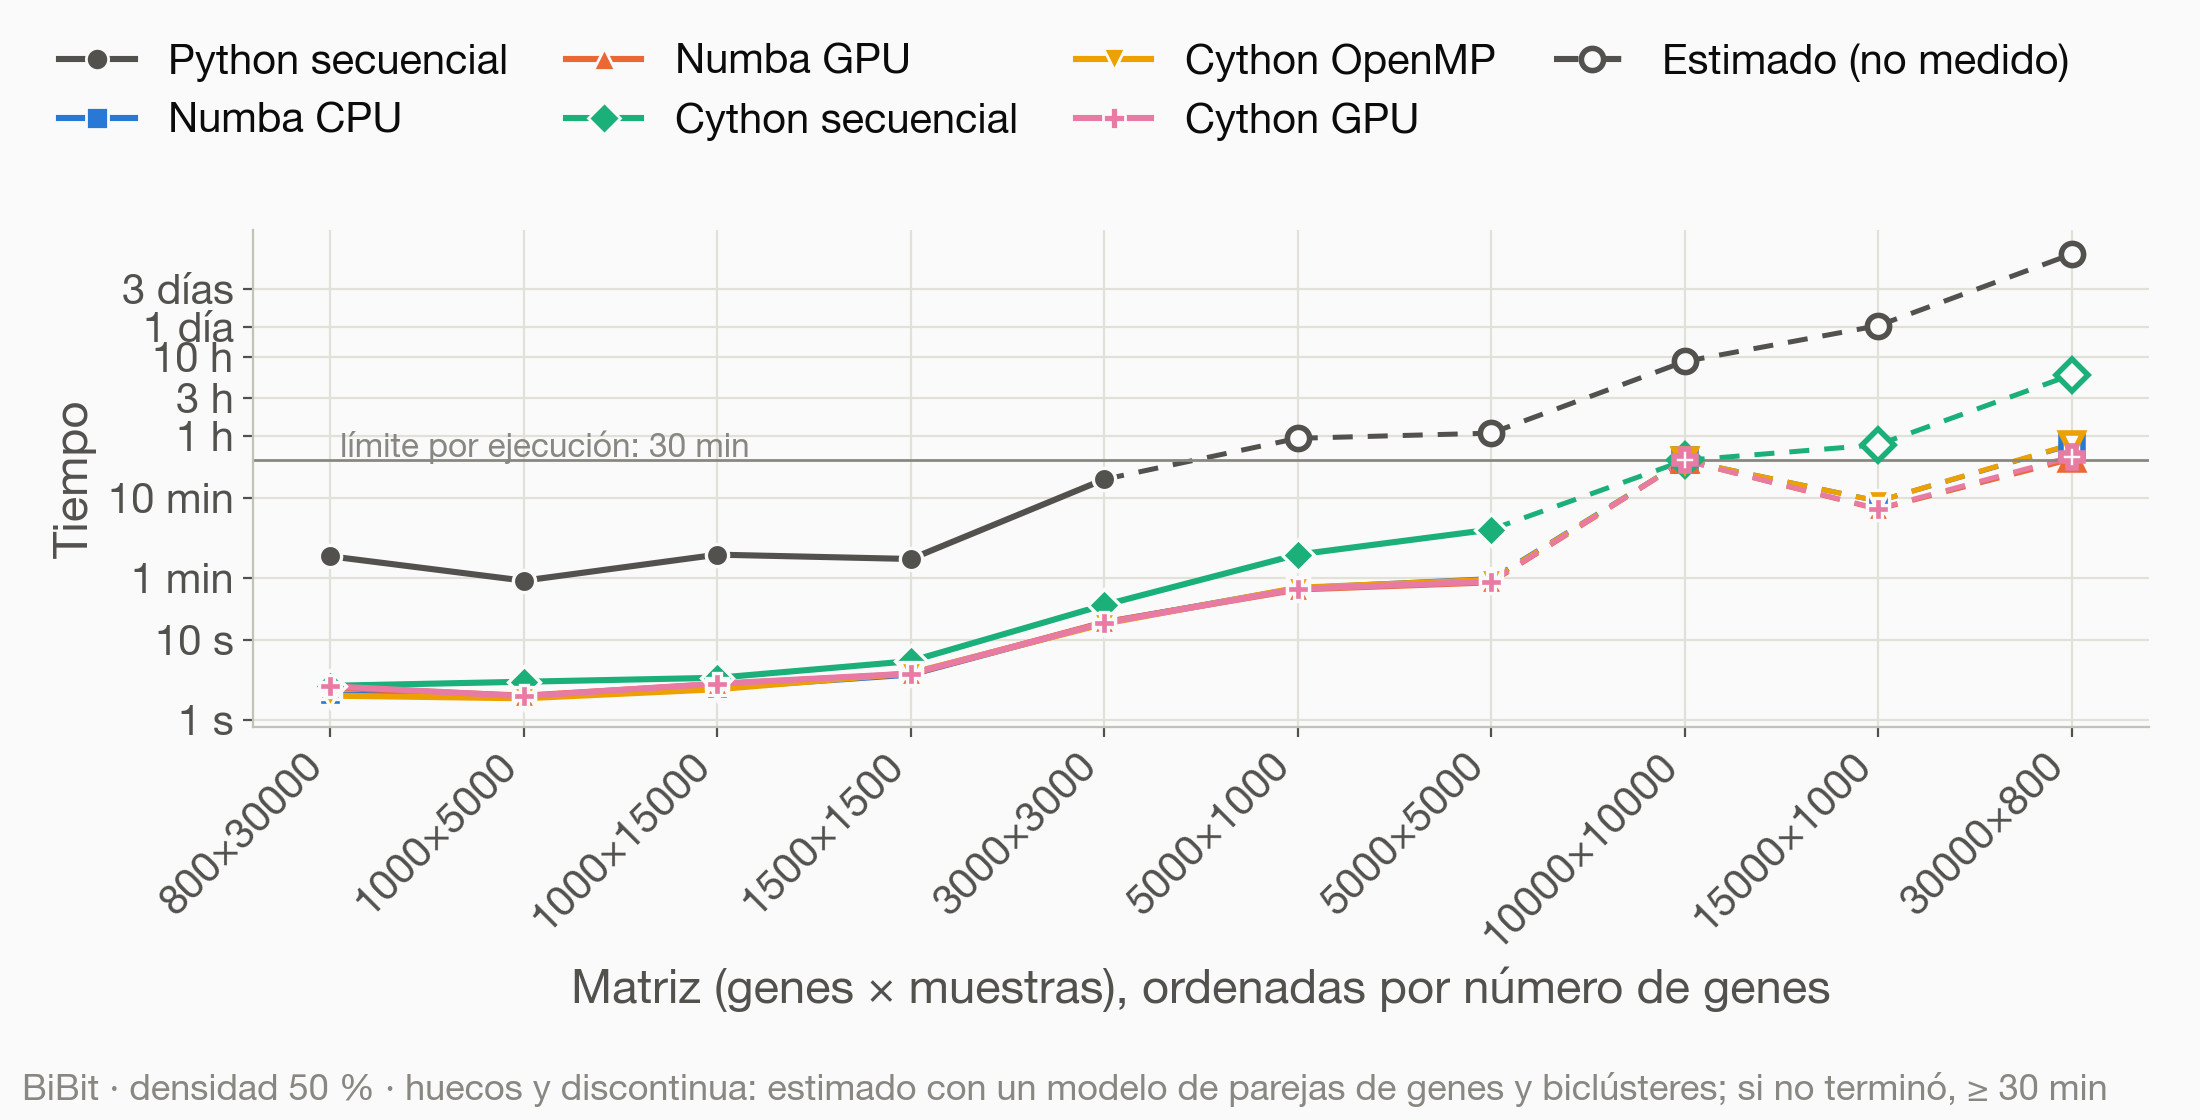
\includegraphics[width=\textwidth,height=0.84\textheight,keepaspectratio]{figuras/resultados/bibit_tiempo_tamano.png}
    \end{center}
\end{frame}

\begin{frame}{BiBit: speedup por modo}
    \begin{center}
        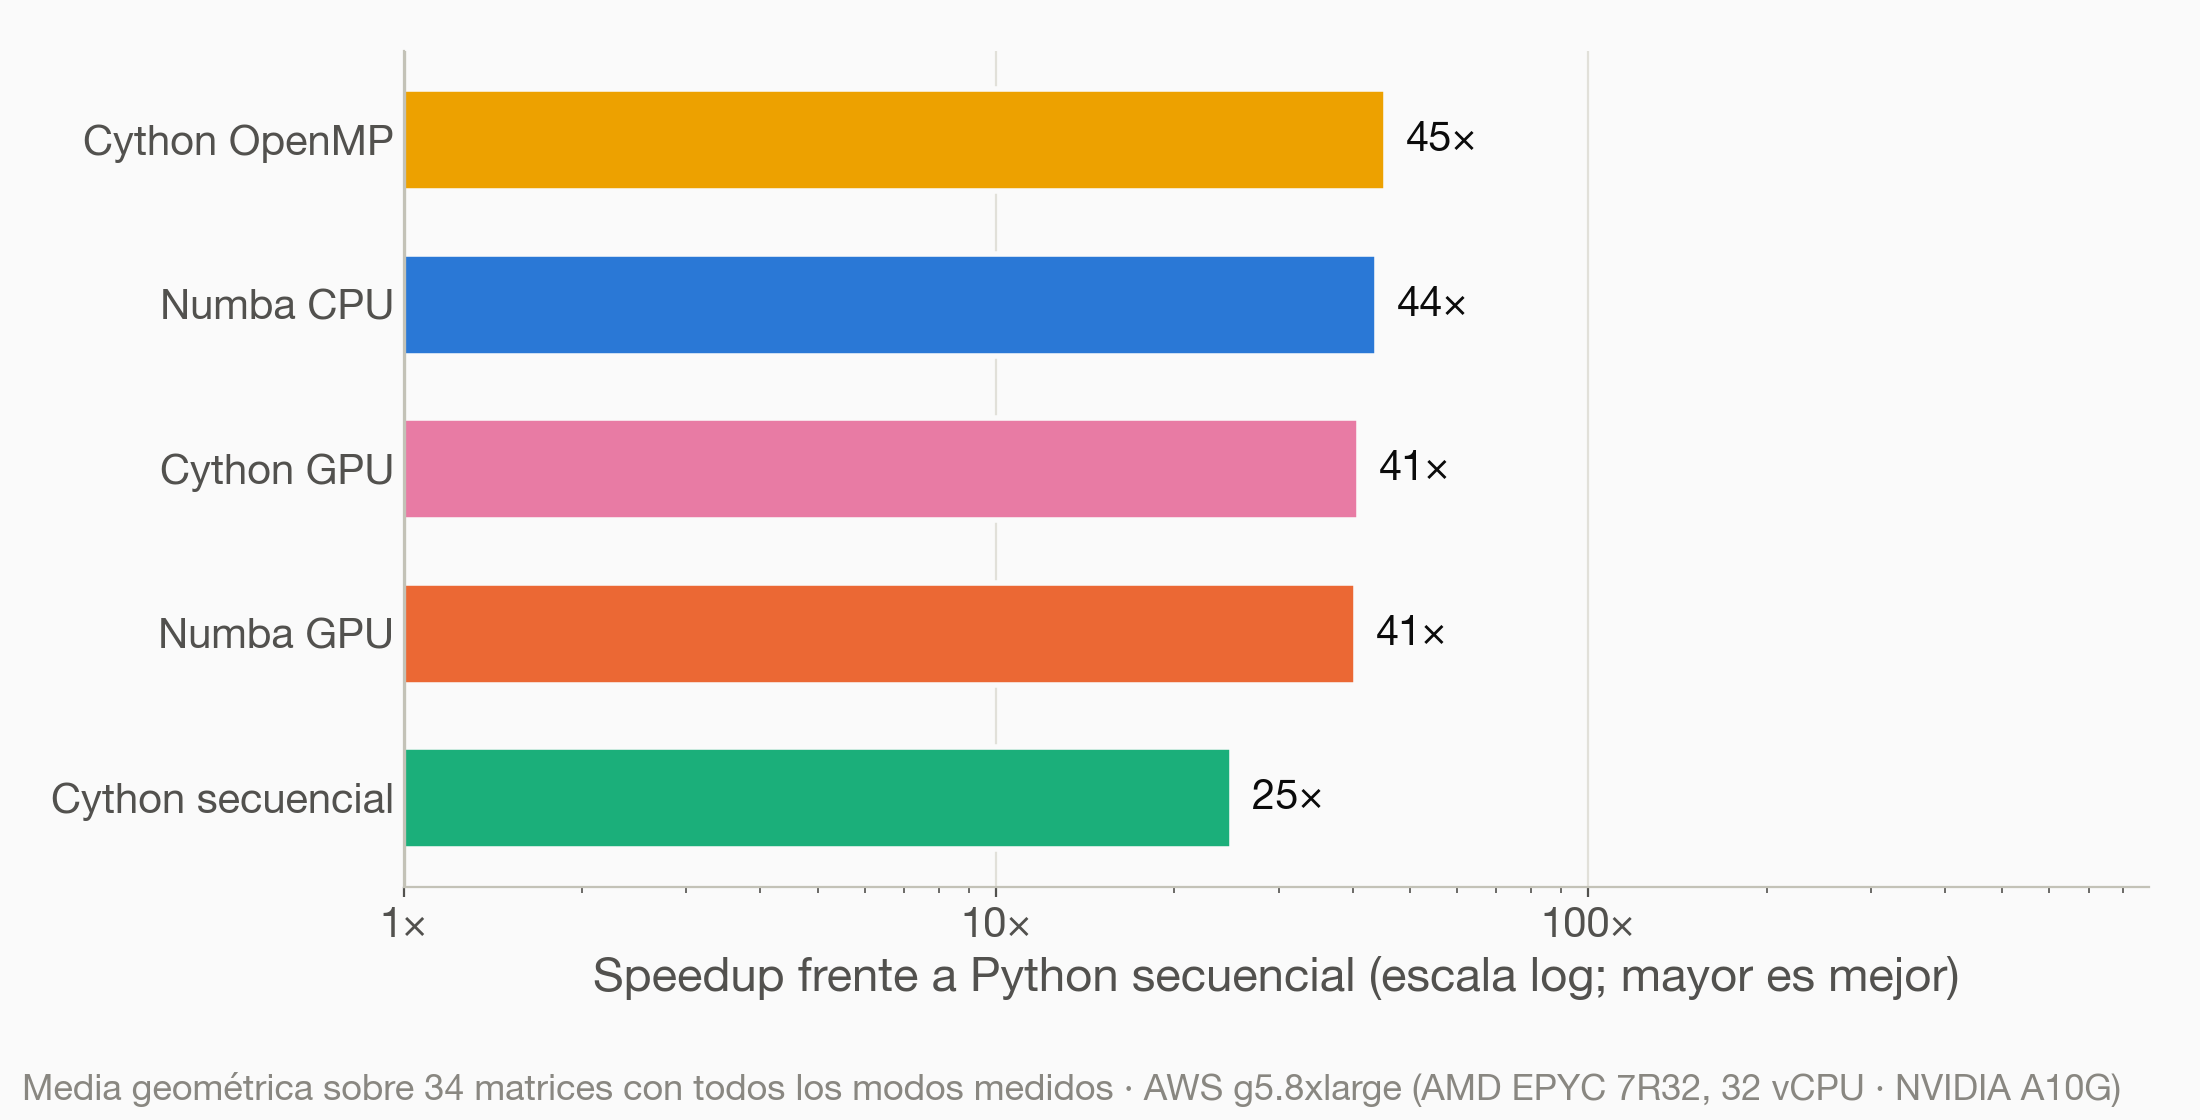
\includegraphics[width=\textwidth,height=0.84\textheight,keepaspectratio]{figuras/resultados/bibit_speedup.png}
    \end{center}
\end{frame}

\begin{frame}{BiBit: speedup por tamaño}
    \begin{center}
        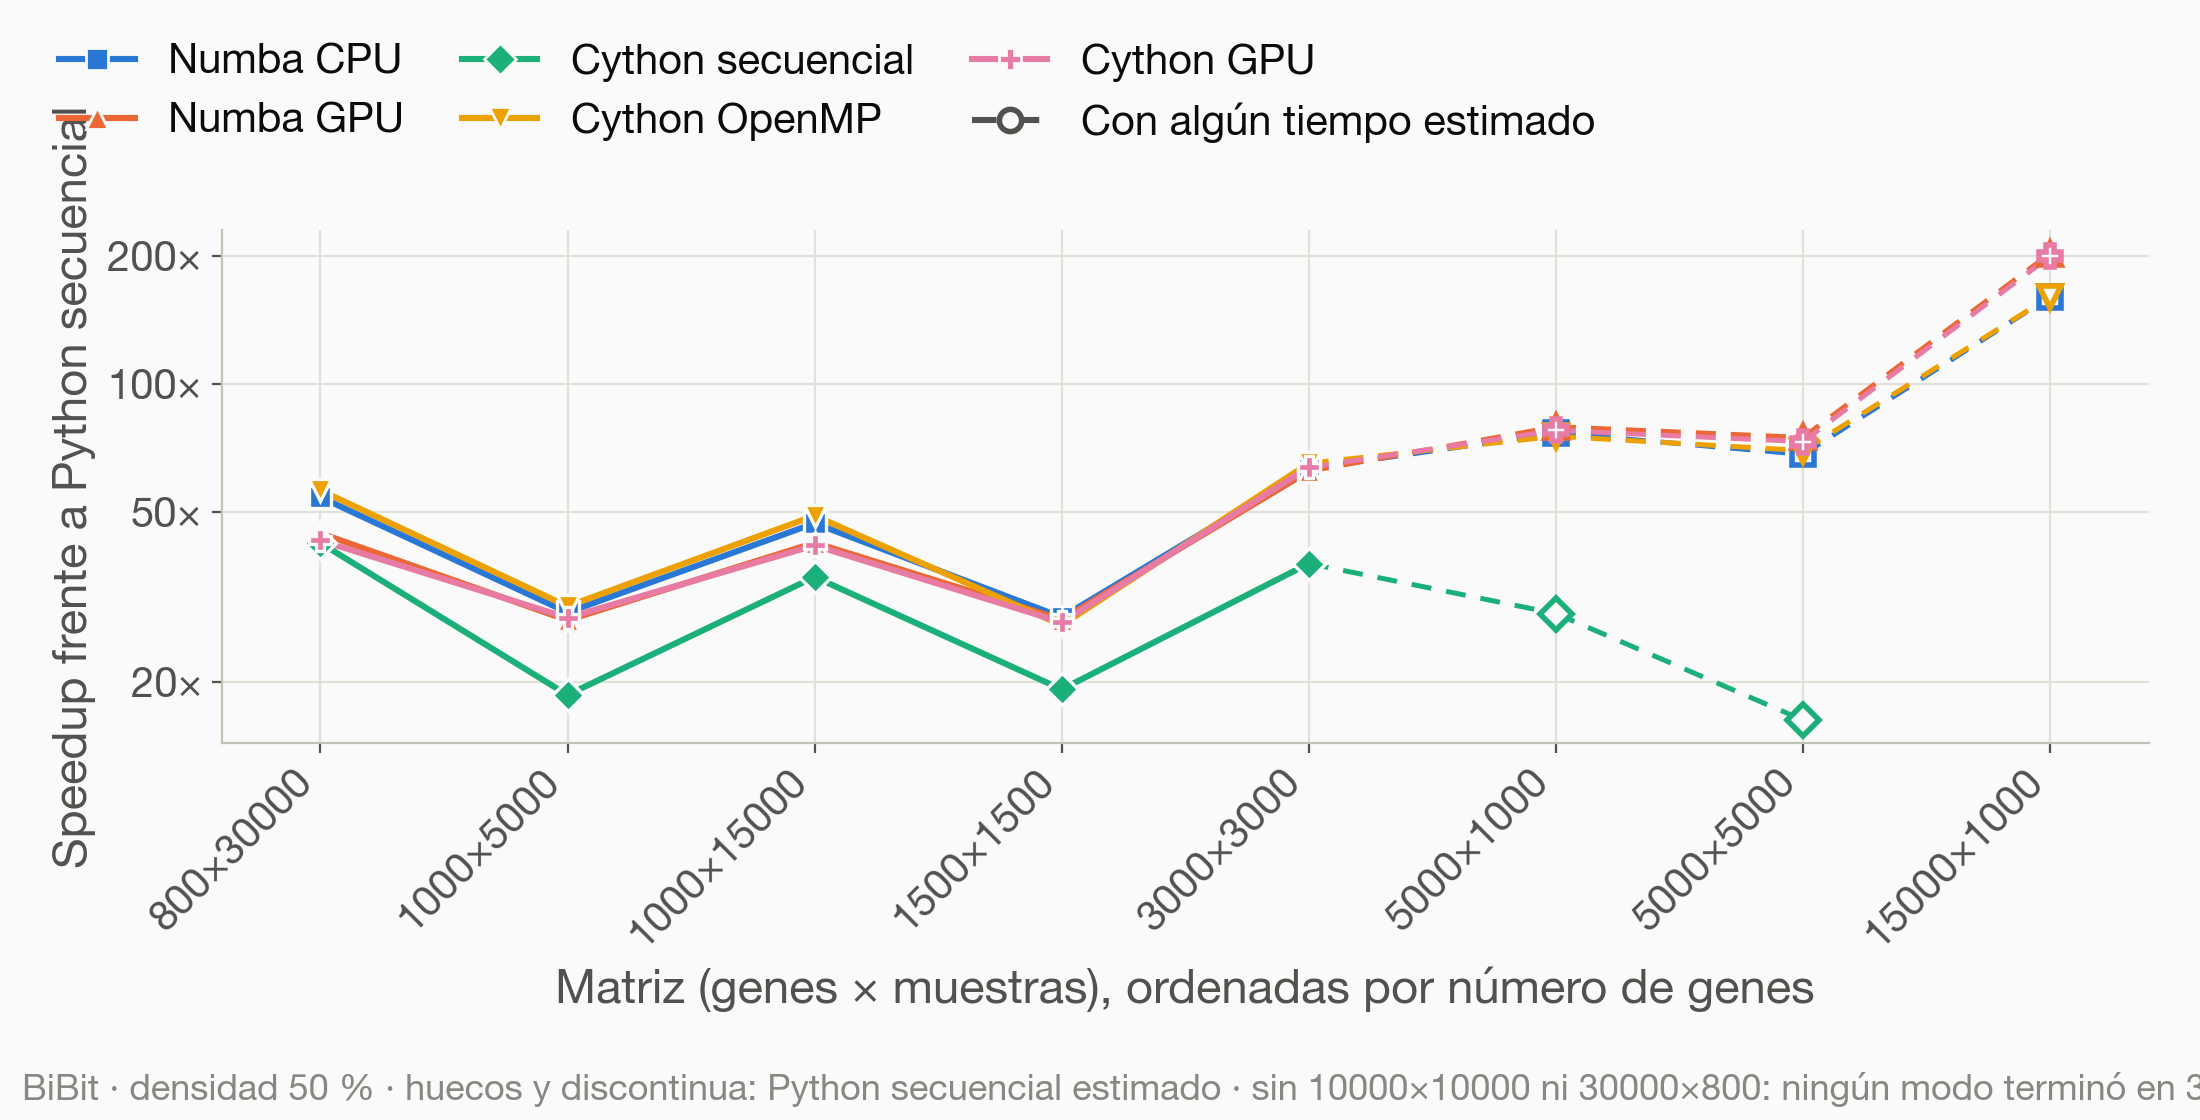
\includegraphics[width=\textwidth,height=0.84\textheight,keepaspectratio]{figuras/resultados/bibit_speedup_tamano.png}
    \end{center}
\end{frame}

\begin{frame}{BCCA: lectura sintética}
    \begin{itemize}
        \item \textbf{Cython GPU:} ganador (252$\times$), seguido de Numba GPU (232$\times$) y Cython OpenMP (230$\times$).
        \item \textbf{Cython secuencial:} 42$\times$ sin un solo hilo.
        \item \textbf{Escalado ordenado:} el tiempo crece con el tamaño (Spearman $\rho \approx 0{,}97$).
    \end{itemize}
\end{frame}

\begin{frame}{BCCA: tiempo mediano por modo}
    \begin{center}
        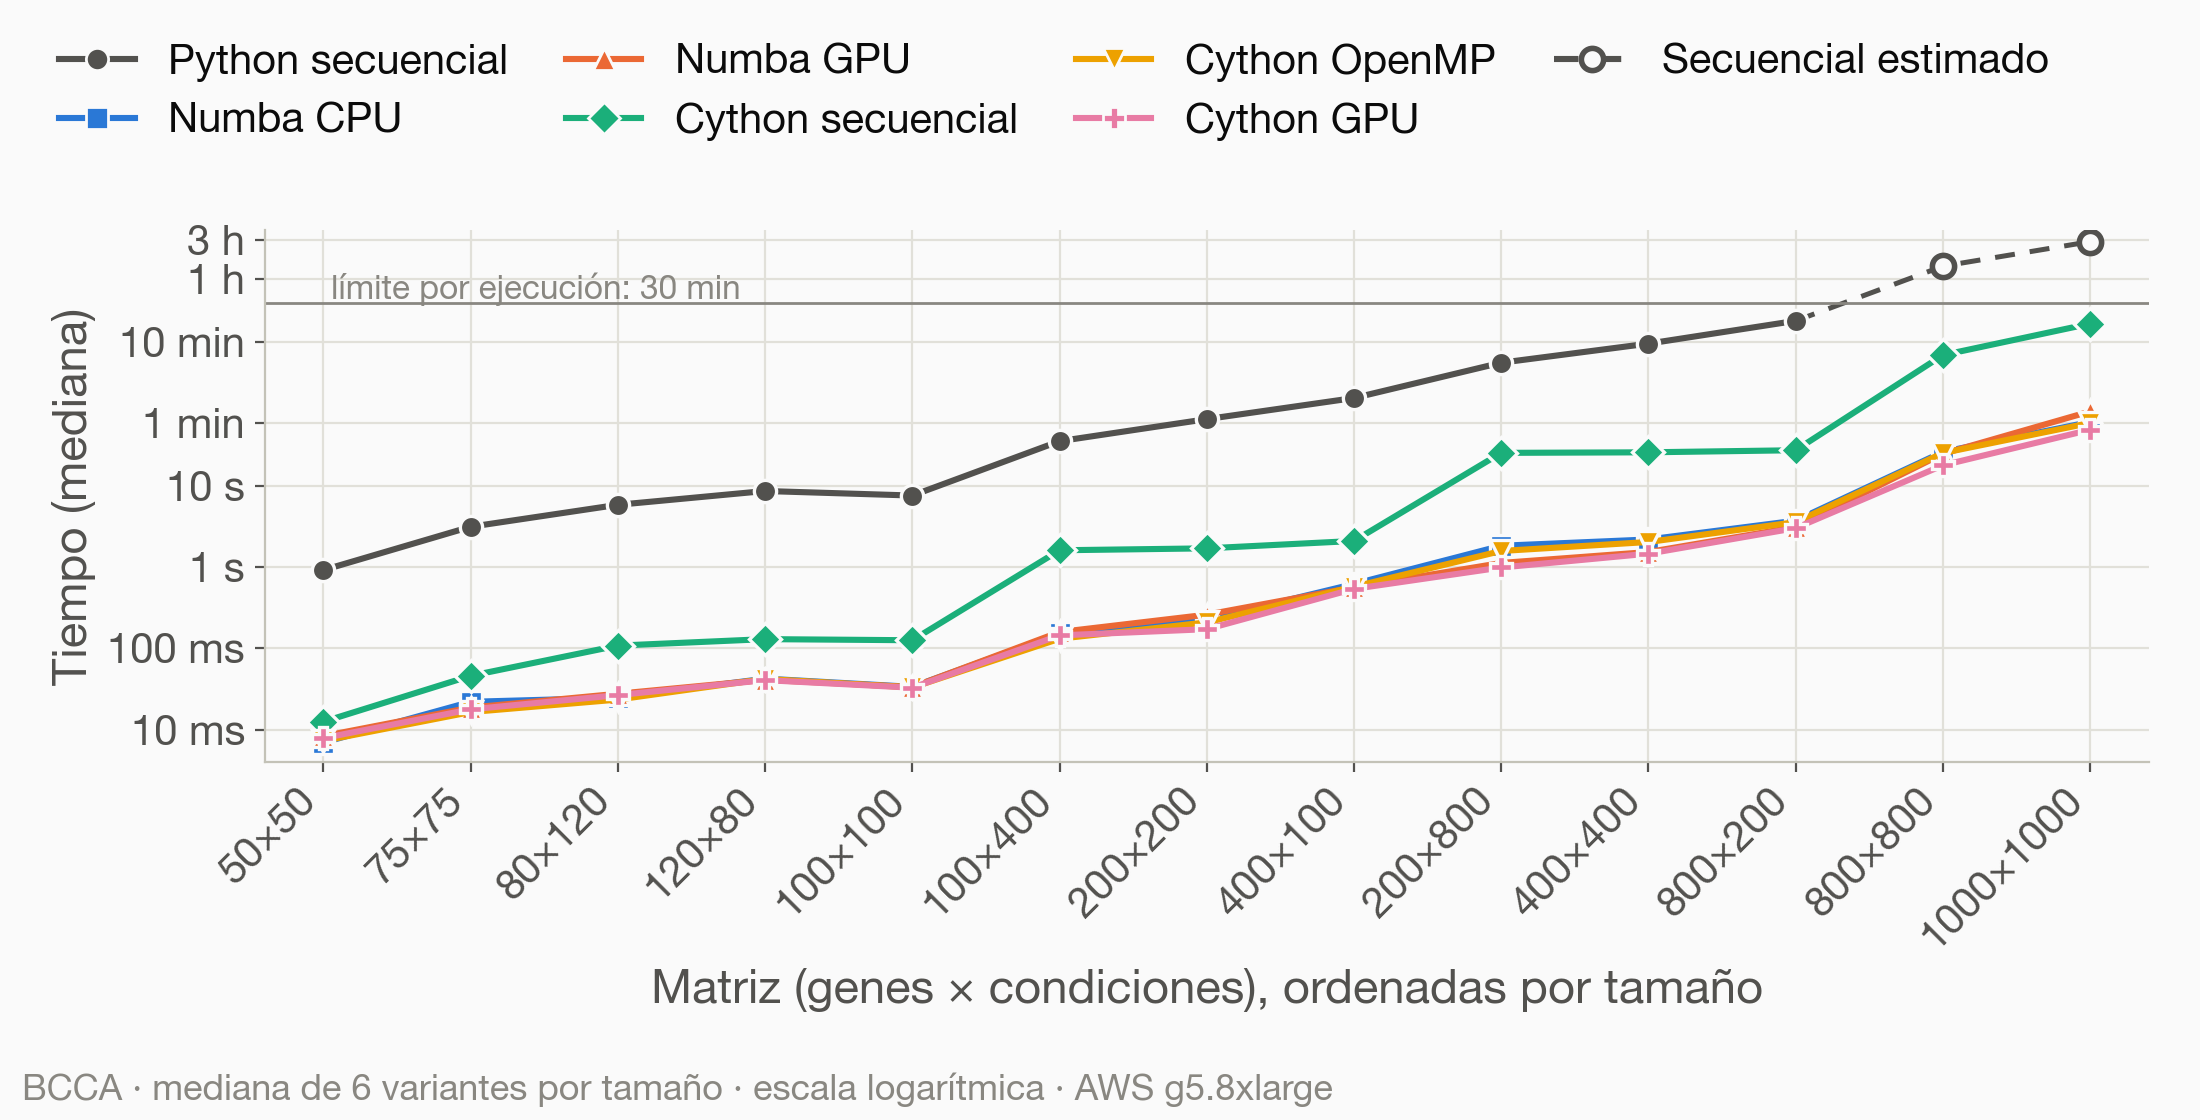
\includegraphics[width=\textwidth,height=0.84\textheight,keepaspectratio]{figuras/resultados/bcca_tiempo_tamano.png}
    \end{center}
\end{frame}

\begin{frame}{BCCA: speedup por modo}
    \begin{center}
        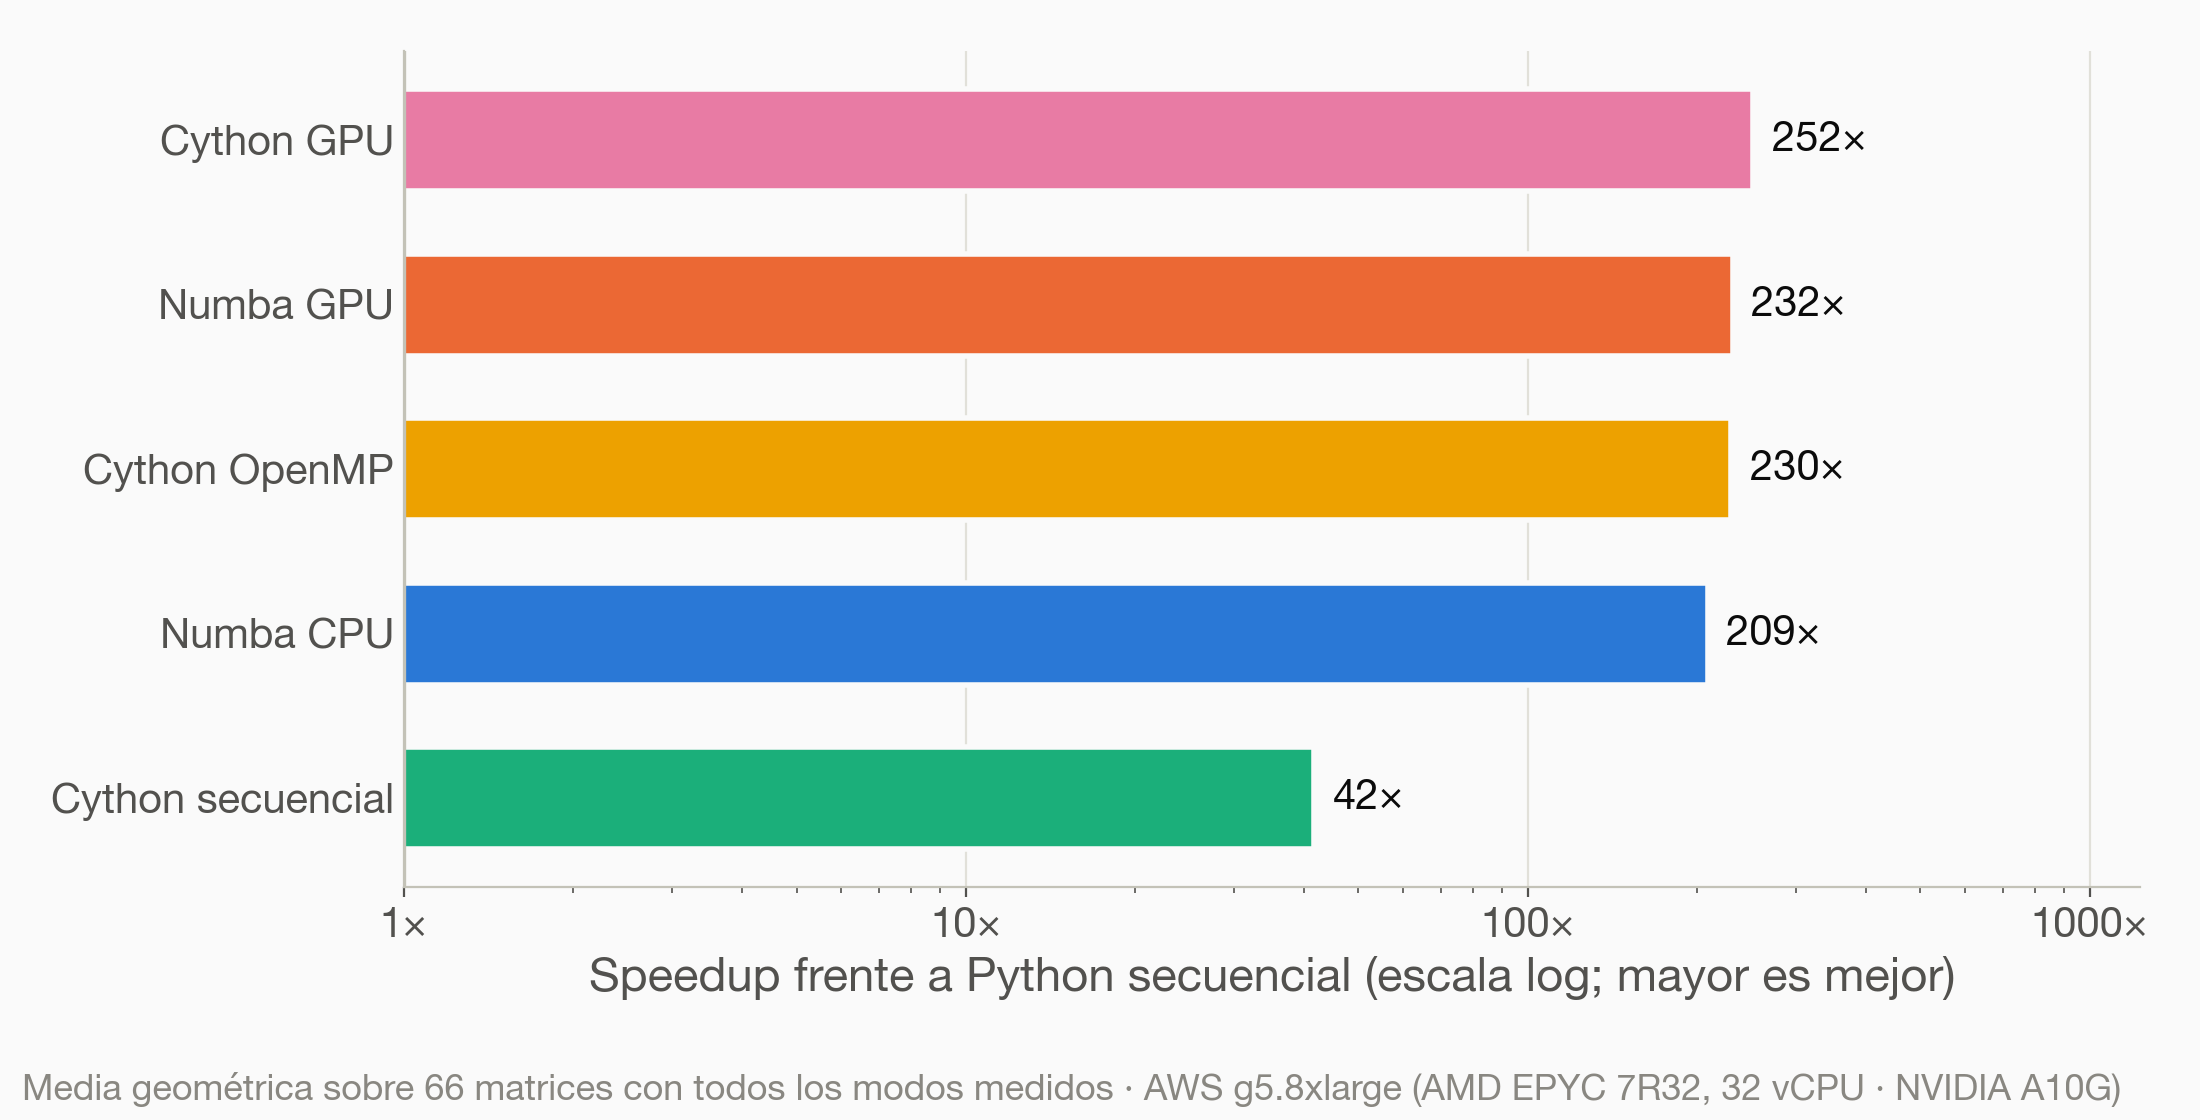
\includegraphics[width=\textwidth,height=0.84\textheight,keepaspectratio]{figuras/resultados/bcca_speedup.png}
    \end{center}
\end{frame}

\begin{frame}{BCCA: speedup por tamaño}
    \begin{center}
        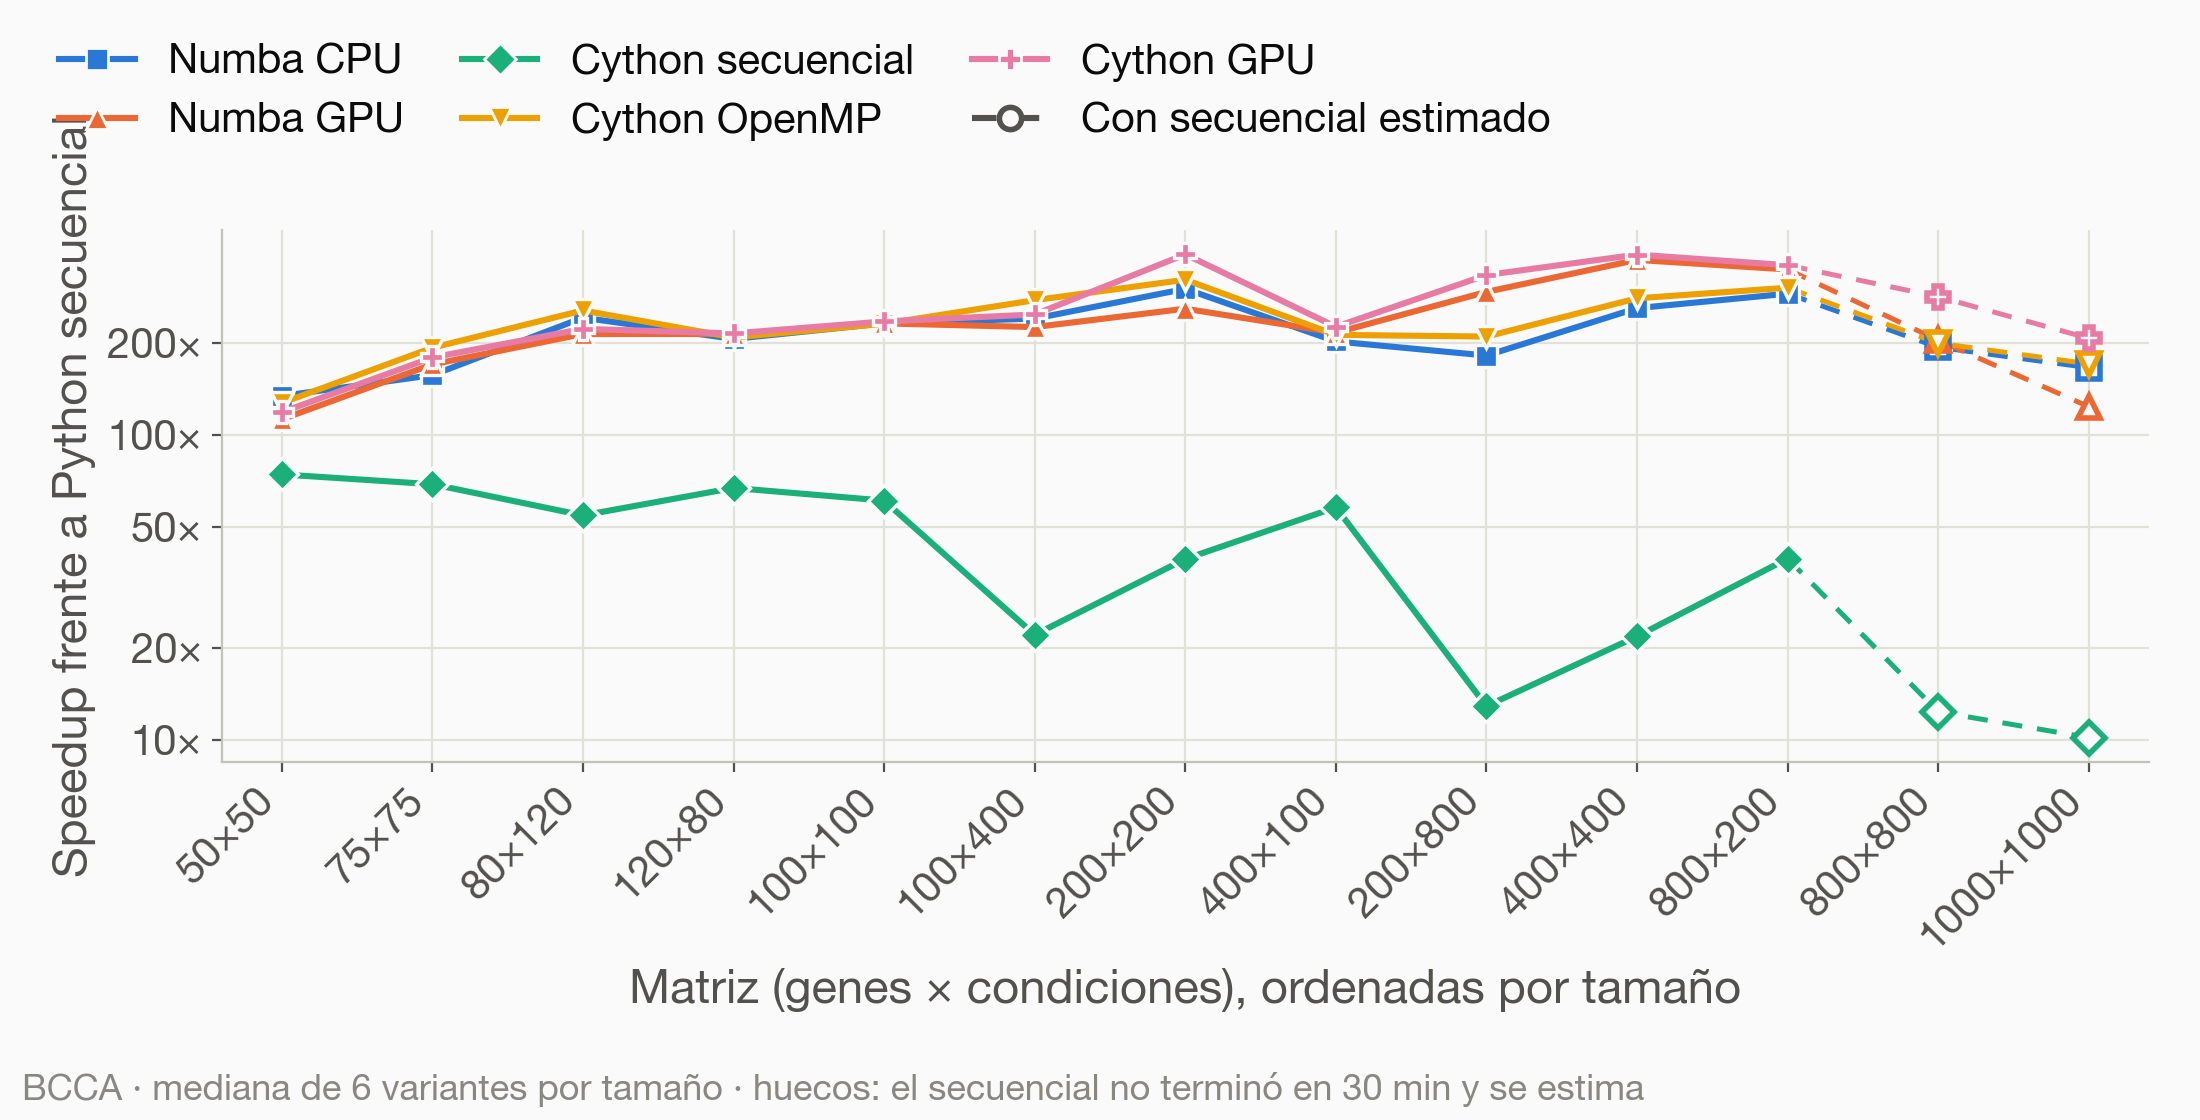
\includegraphics[width=\textwidth,height=0.84\textheight,keepaspectratio]{figuras/resultados/bcca_speedup_tamano.png}
    \end{center}
\end{frame}

\begin{frame}{BiBit vs.\ BCCA: mismo paradigma, distinto efecto}
    \begin{center}
        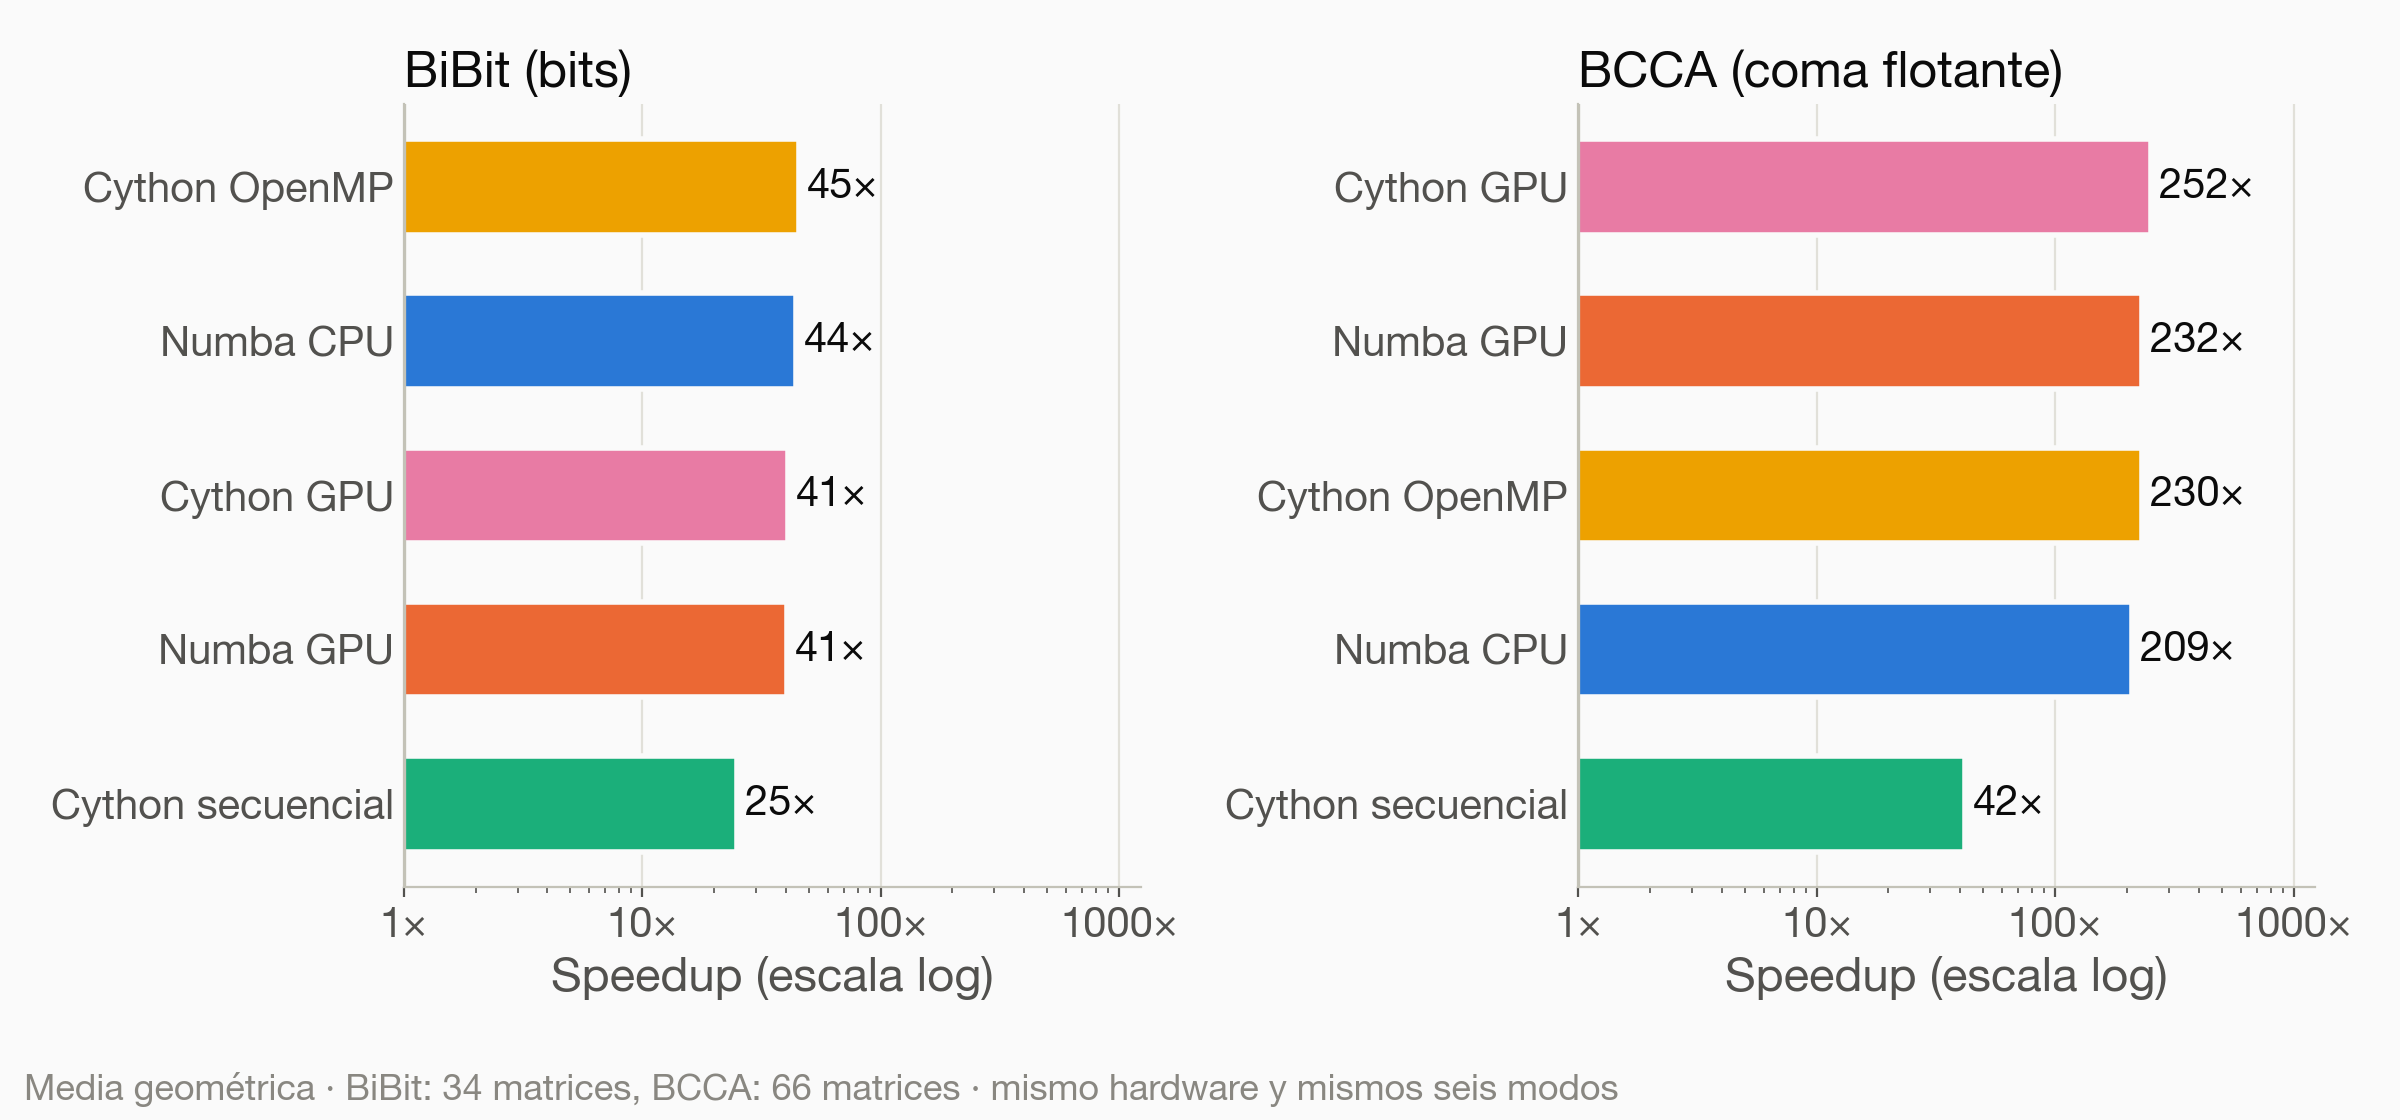
\includegraphics[width=\textwidth,height=0.84\textheight,keepaspectratio]{figuras/resultados/comparativa_speedup.png}
    \end{center}
\end{frame}

\begin{frame}{Complejidad de implementación}
    \begin{table}
        \centering
        \renewcommand{\arraystretch}{1.15}
        \resizebox{0.62\textwidth}{!}{
        \begin{tabular}{@{}lccl@{}}
            \toprule
            \textbf{Variante} & \textbf{BiBit} & \textbf{BCCA} & \textbf{Herramientas necesarias} \\ \midrule
            Python secuencial & 26 & 40 & Python + NumPy \\
            Numba CPU & 94 & 80 & + \texttt{numba} \\
            Numba GPU & 139 & 96 & + \textit{driver} CUDA \\
            Cython secuencial & 134$^{*}$ & 115$^{*}$ & + compilador C \\
            Cython OpenMP & 134$^{*}$ & 115$^{*}$ & + OpenMP \\
            Cython GPU & 257 & 146 & + \texttt{nvcc} y CUDA C/C++ \\
            \bottomrule
        \end{tabular}
        }
    \end{table}
    \vspace{-0.1cm}
    {\footnotesize Líneas de código propias de cada variante (sin comentarios ni líneas en blanco). $^{*}$Secuencial y OpenMP comparten el mismo módulo.\par}
    \vspace{0.2cm}
    \begin{itemize}
        \item \textbf{Numba CPU:} 2--3,6$\times$ más código que el secuencial; 44$\times$ en BiBit y 209$\times$ en BCCA.
        \item \textbf{Cython GPU en BCCA:} $\sim$3,7$\times$ más código y tres lenguajes por 252$\times$.
    \end{itemize}
\end{frame}

\begin{frame}{Resumen estadístico}
    \begin{table}
        \centering
        \renewcommand{\arraystretch}{1.4}
        \resizebox{0.85\textwidth}{!}{
        \begin{tabular}{@{}lcc@{}}
            \toprule
             & \textbf{BiBit} & \textbf{BCCA} \\ \midrule
            \textbf{Friedman} ($\chi^2$, $p$) & 135,82; $1{,}4\cdot10^{-27}$ & 258,64; $7{,}7\cdot10^{-54}$ \\
            \textbf{Kendall W} & 0,80 (acuerdo fuerte) & 0,78 (acuerdo fuerte) \\
            \textbf{Wilcoxon vs secuencial} & $p \approx 1{,}2\cdot10^{-10}$ en todos & $p \approx 1{,}6\cdot10^{-12}$ en todos \\
            \textbf{Datasets donde gana el modo} & 100\,\% & 100\,\% \\
            \textbf{Spearman $\rho$ (tamaño--tiempo)} & 0,17 -- 0,38 & 0,96 -- 0,98 \\
            \textbf{Mejor modo} & Cython OpenMP (45$\times$) & Cython GPU (252$\times$) \\
            \bottomrule
        \end{tabular}
        }
    \end{table}
    {\footnotesize Matrices con los seis modos medidos: 34 en BiBit y 66 en BCCA (límite de 30\,min por ejecución).\par}
\end{frame}

% --- SECCIÓN 5: CONCLUSIONES ---
\begin{frame}[plain]
    \begin{tikzpicture}[remember picture,overlay]
        \fill[black!2] (current page.south west) rectangle (current page.north east);
        \fill[blue!72!black] (current page.north west) rectangle ([xshift=0.36cm]current page.south west);
        \fill[blue!72!black] ([xshift=0.36cm]current page.south west) rectangle ([yshift=0.16cm]current page.south east);
        \node[anchor=west, text=blue!72!black, font=\bfseries\Large] at ([xshift=1.25cm,yshift=-1.4cm]current page.north west) {BLOQUE 5/5};
        \node[anchor=west, align=left, text width=13.5cm, text=black, font=\bfseries\fontsize{24}{28}\selectfont] at ([xshift=1.25cm,yshift=-3.35cm]current page.north west) {Conclusiones e ingeniería};
        \draw[blue!72!black, line width=1pt] ([xshift=1.25cm,yshift=-5.25cm]current page.north west) -- ([xshift=10.9cm,yshift=-5.25cm]current page.north west);
        \node[anchor=west, align=left, text width=13.5cm, text=black!65, font=\large] at ([xshift=1.25cm,yshift=-6.25cm]current page.north west) {La respuesta: dónde está el límite de Python y cuándo bajar a C.};
    \end{tikzpicture}
\end{frame}

\section{Conclusiones y recomendaciones de ingeniería}



\begin{frame}{¿Cuál es el límite de Python?}
    \begin{center}
    \begin{tikzpicture}[
        card/.style={rounded corners=1ex, very thick, minimum width=4.8cm, minimum height=2.6cm, align=center}
    ]
        \node[card, draw=red!60!black, fill=red!8] (py) at (-3.1,0) {
            {\small\bfseries Python secuencial}\\[0.4em]
            {\fontsize{22}{24}\selectfont\bfseries 18 min}\\[0.3em]
            {\footnotesize 1\,097 s}
        };
        \node[card, draw=green!45!black, fill=green!10] (cu) at (3.1,0) {
            {\small\bfseries Cython + CUDA}\\[0.4em]
            {\fontsize{22}{24}\selectfont\bfseries 3 s}\\[0.3em]
            {\footnotesize 3,05 s}
        };
        \draw[-{Stealth[length=4mm]}, line width=2pt, black!60] (py.east) -- (cu.west);
        \node[font=\small\bfseries] at (0,-1.75) {BCCA, matriz real de solo 800 $\times$ 200};
    \end{tikzpicture}
    \end{center}
    \vspace{0.1cm}
    \begin{itemize}
        \item \textbf{El límite no es el lenguaje:} es el intérprete ejecutando bucles numéricos.
        \item \textbf{Python orquesta, C/CUDA calcula:} el techo pasa a ser el hardware.
    \end{itemize}
\end{frame}

\begin{frame}{Guía rápida de decisión}
    \begin{center}
    \resizebox{0.8\textwidth}{!}{
    \begin{tikzpicture}[
        q/.style={draw=blue!60, fill=blue!10, rounded corners=1ex, very thick, align=center, minimum width=4.2cm, minimum height=1cm, font=\small\bfseries},
        a/.style={draw=green!50!black, fill=green!12, rounded corners=1ex, very thick, align=center, minimum width=3.2cm, minimum height=0.9cm, font=\small},
        arrow/.style={-{Stealth[length=3mm]}, line width=1.2pt, black!70},
        lbl/.style={font=\scriptsize\bfseries, fill=white, inner sep=1pt}
    ]
        \node[q] (q1) at (0,0) {¿El tiempo importa\\en la práctica?};
        \node[a] (a1) at (5,0) {Python + NumPy};
        \node[q] (q2) at (0,-1.8) {¿Bucles con NumPy\\simple?};
        \node[a] (a2) at (5,-1.8) {Numba CPU};
        \node[q] (q3) at (0,-3.6) {¿Problema masivo y\\muy paralelo?};
        \node[a] (a3) at (-5,-3.6) {Cython + OpenMP};
        \node[q] (q4) at (0,-5.4) {¿Aritmética densa y\\distribución controlada?};
        \node[a] (a4) at (5,-5.4) {Cython + CUDA};
        \node[a] (a5) at (-5,-5.4) {Numba CUDA};

        \draw[arrow] (q1) -- node[lbl] {no} (a1);
        \draw[arrow] (q1) -- node[lbl] {sí} (q2);
        \draw[arrow] (q2) -- node[lbl] {sí} (a2);
        \draw[arrow] (q2) -- node[lbl] {no} (q3);
        \draw[arrow] (q3) -- node[lbl] {no} (a3);
        \draw[arrow] (q3) -- node[lbl] {sí} (q4);
        \draw[arrow] (q4) -- node[lbl] {sí} (a4);
        \draw[arrow] (q4) -- node[lbl] {no} (a5);
    \end{tikzpicture}
    }
    \end{center}
\end{frame}

\begin{frame}[plain]
    \begin{tikzpicture}[remember picture,overlay]
        \fill[black!2] (current page.south west) rectangle (current page.north east);
        \fill[orange!85!black] (current page.north west) rectangle ([xshift=0.36cm]current page.south west);
        \node[anchor=west, align=left, text width=13.5cm, text=black, font=\bfseries\fontsize{22}{27}\selectfont] at ([xshift=1.25cm,yshift=-2.1cm]current page.north west) {Bajar a C da miedo.\\A veces es imprescindible.};
        \draw[orange!85!black, line width=1pt] ([xshift=1.25cm,yshift=-3.55cm]current page.north west) -- ([xshift=10.9cm,yshift=-3.55cm]current page.north west);
        \node[anchor=north west, align=left, text width=13.5cm, text=black!75, font=\large] at ([xshift=1.25cm,yshift=-3.9cm]current page.north west) {
            $\bullet$ No hay que reescribirlo todo: solo el núcleo caliente.\\[0.5em]
            $\bullet$ El usuario sigue en Python: \texttt{bs.bcca(dataset, mode=6)}.\\[0.5em]
            $\bullet$ BCCA: 146 líneas de Cython + CUDA $\rightarrow$ 252$\times$.\\[0.5em]
            $\bullet$ De un experimento inviable a uno rutinario.
        };
    \end{tikzpicture}
\end{frame}

\begin{frame}[plain]
    \begin{tikzpicture}[remember picture,overlay]
        \fill[black!2] (current page.south west) rectangle (current page.north east);
        \fill[blue!72!black] (current page.north west) rectangle ([xshift=0.36cm]current page.south west);
        \node[anchor=west, text=blue!72!black, font=\bfseries\fontsize{30}{34}\selectfont] at ([xshift=1.3cm,yshift=-2.1cm]current page.north west) {¿Preguntas?};
        \draw[blue!72!black, line width=1pt] ([xshift=1.3cm,yshift=-3.05cm]current page.north west) -- ([xshift=8.7cm,yshift=-3.05cm]current page.north west);
        \node[anchor=west, text=black!78, font=\Large] at ([xshift=1.3cm,yshift=-4.25cm]current page.north west) {\textbf{Pablo Oca}};
        \node[anchor=west, text=black!62, font=\large] at ([xshift=1.3cm,yshift=-4.95cm]current page.north west) {\texttt{pabloocagal03@gmail.com}};
    \end{tikzpicture}
\end{frame}

\end{document}